% ============================================================
%  Shared preamble - matches the Mode-0/1/2 report house style
% ============================================================
\documentclass[11pt,a4paper]{article}

\usepackage[utf8]{inputenc}
\usepackage[expansion=false]{microtype}
\usepackage[a4paper,left=28mm,right=28mm,top=28mm,bottom=25mm]{geometry}

\usepackage{amsmath,amssymb}
\usepackage{booktabs}
\usepackage{array}
\usepackage{enumitem}
\usepackage{xcolor}
\usepackage{caption}
\usepackage{fancyhdr}
\usepackage{titlesec}
\usepackage{tikz}
\usetikzlibrary{positioning,arrows.meta,calc,fit,backgrounds,shapes.geometric,decorations.pathreplacing}
\usepackage[most]{tcolorbox}
\usepackage[section]{placeins}
\usepackage[hidelinks]{hyperref}

% ---------- colours ----------
\definecolor{navy}{RGB}{26,60,102}
\definecolor{accent}{RGB}{40,92,148}
\definecolor{softblue}{RGB}{232,240,248}
\definecolor{rulegrey}{RGB}{120,130,140}
\definecolor{orangeacc}{RGB}{196,106,48}
\definecolor{boxblue}{RGB}{219,232,244}
\definecolor{tealbox}{RGB}{214,236,238}
\definecolor{peachbox}{RGB}{250,226,208}
\definecolor{pinkbox}{RGB}{247,222,226}
\definecolor{greenbox}{RGB}{223,238,224}
\definecolor{greybox}{RGB}{238,240,242}

\hypersetup{
  colorlinks=true,
  linkcolor=accent,
  urlcolor=accent,
  citecolor=accent,
  pdftitle={Bluetooth Channel Sounding Campaign Configuration and Scheduling},
  pdfsubject={Formal technical report},
}

% ---------- headings ----------
\titleformat{\section}{\normalfont\Large\bfseries\color{navy}}{\thesection}{0.8em}{}
\titleformat{\subsection}{\normalfont\large\bfseries\color{navy}}{\thesubsection}{0.7em}{}
\titleformat{\subsubsection}{\normalfont\normalsize\bfseries\color{navy}}{\thesubsubsection}{0.6em}{}
\titlespacing*{\section}{0pt}{1.9\baselineskip}{0.8\baselineskip}
\titlespacing*{\subsection}{0pt}{1.2\baselineskip}{0.5\baselineskip}

% ---------- captions ----------
\captionsetup{font=small,labelfont={bf,color=accent},labelsep=colon,width=0.92\textwidth}
\captionsetup[table]{position=above,skip=4pt}
\captionsetup[figure]{position=below,skip=8pt}

% ---------- headers ----------
\pagestyle{fancy}
\fancyhf{}
\renewcommand{\headrulewidth}{0.6pt}
\fancyhead[L]{\small Bluetooth CS Campaign Configuration and Scheduling}
\fancyhead[R]{\small Formal technical report - Revision 1.0}
\fancyfoot[C]{\small\thepage}

% ---------- callout box ----------
\newtcolorbox{callout}[1][]{
  colback=softblue, colframe=accent, boxrule=0.5pt,
  left=6pt,right=6pt,top=5pt,bottom=5pt, arc=1pt,
  fontupper=\small, #1}

% ---------- table helpers ----------
\newcolumntype{L}[1]{>{\raggedright\arraybackslash}p{#1}}
\newcolumntype{C}[1]{>{\centering\arraybackslash}p{#1}}
\renewcommand{\arraystretch}{1.18}
\emergencystretch=3em

% ---------- macros ----------
\newcommand{\us}{\,\ensuremath{\upmu}s}
\newcommand{\code}[1]{\texttt{\small #1}}
\newcommand{\FFO}{\mathrm{FFO}}
\newcommand{\ToF}{\mathrm{ToF}}
\newcommand{\RTT}{\mathrm{RTT}}
\newcommand{\PCT}{\mathrm{PCT}}
\newcommand{\Tsy}{T_{SY}}
\newcommand{\Trd}{T_{RD}}
\newcommand{\Tip}{T_{IP1}}
\newcommand{\Tipp}{T_{IP2}}
\newcommand{\Tfcs}{T_{FCS}}
\newcommand{\Tgd}{T_{GD}}
\newcommand{\Tfm}{T_{FM}}
\newcommand{\Tsw}{T_{SW}}
\newcommand{\Tpm}{T_{PM}}
\newcommand{\Nap}{N_{AP}}
\newcommand{\Tconn}{T_{C}}
\newcommand{\Tse}{T_{SE}}
\newcommand{\Tsei}{T_{SEI}}
\newcommand{\Nse}{N_{SE}}
\newcommand{\Nei}{N_{EI}}
\newcommand{\Npi}{N_{PI}}
\newcommand{\Npc}{N_{PC}}
\newcommand{\Tpl}{T_{PL}}
\newcommand{\Nst}{N_{step}}
\providecommand{\upmu}{\mu}

% Core specification citation shorthand
\newcommand{\core}[1]{\textcolor{rulegrey}{\small[Core 6.3, #1]}}

% TikZ block styles reused across figures
\tikzset{
  blk/.style   ={draw=navy!70, fill=softblue, rounded corners=1pt, align=center,
                 font=\scriptsize, inner sep=3.5pt, minimum height=8mm},
  pblk/.style  ={draw=navy!70, fill=white, rounded corners=1pt, align=center,
                 font=\scriptsize, inner sep=3.5pt, minimum height=8mm},
  ar/.style    ={-{Latex[length=2mm]}, draw=navy!80, thick},
  dar/.style   ={-{Latex[length=2mm]}, draw=orangeacc, dashed, thin},
  slot/.style  ={draw=navy!55, font=\scriptsize, align=center, minimum height=7mm},
}

% ============================================================
\begin{document}

% ---------------- Title page ----------------
\thispagestyle{empty}
\vspace*{18mm}
{\color{accent}\small\bfseries FORMAL TECHNICAL REPORT \hfill REVISION 1.0}

\vspace{26mm}
{\raggedright\color{navy}\Huge\bfseries Bluetooth Channel Sounding\par}
\vspace{5mm}
{\raggedright\color{navy}\huge\bfseries Campaign Configuration and Scheduling\par}

\vspace{7mm}
\noindent{\raggedright\color{rulegrey}\large Capability negotiation, configuration and procedure
parameters, ACL anchoring, and the procedure--event--subevent--step hierarchy\par}

\vspace{12mm}
\noindent\rule{\textwidth}{1pt}

\vspace{4mm}
\noindent
The three companion reports treat the single CS step: what Mode-0, Mode-1 and Mode-2 measure and how
the measurement is estimated. This report treats everything that surrounds the step. It follows the
configuration lifecycle from capability exchange through security establishment, configuration
creation, channel classification and procedure parameters to procedure enable, identifying at each
stage which parameters are negotiated with the peer over the ACL connection, which are purely local,
and which are \emph{answered} by the Controller rather than requested by the Host. It then shows how
the ACL connection enters the schedule: as the time base whose anchor points every CS event hangs
from, as the unit in which event and procedure intervals are counted, as the source of the security
context from which the CS nonce material is derived, and as the supervision relationship whose loss
terminates the campaign. The scheduling hierarchy is then developed level by level -- campaign,
procedure, event, subevent, step -- with the ordering rules that place Mode-0, main mode and sub mode
steps inside a subevent, the step-duration arithmetic for all four modes, and the capacity
calculation that converts a subevent length into a step count. A worked example carries one complete
configuration from Host parameters to measurement rate, duty cycle and channel coverage. Coexistence,
result reporting, campaign-level error sources, a verification plan and an HCI parameter appendix
close the report.

\vfill
\noindent
\begin{tabular}{@{}L{40mm}L{95mm}@{}}
Primary references & Core 6.3, Vol.\ 6, Part H, Secs.\ 4.1--4.2 and 4.5; Vol.\ 6, Part B, CS Link
                     Layer control procedures \\
Host interface & Core 6.3, Vol.\ 4, Part E, LE CS command and event set \\
Companion reports & \emph{Bluetooth CS Mode-0 Frequency Estimation}, Revision 3.0;
                    \emph{Bluetooth CS Mode-1 RTT Estimation}, Revision 1.0;
                    \emph{Bluetooth CS Mode-2 Phase-Based Ranging}, Revision 1.0 \\
Document type & Scientific and implementation-oriented technical report \\
Revision date & 4 September 2026 \\
\end{tabular}

\newpage
\pagenumbering{roman}

% ---------------- Abstract ----------------
\section*{Abstract}
\addcontentsline{toc}{section}{Abstract}

A Channel Sounding measurement campaign is the outer envelope of everything the mode reports
describe. The individual step is where a frequency, a time or a phase is measured; but how many steps
run, which channels they occupy, at what instants they occur, how many of them share a coherent
frequency reference, and how often the whole pattern repeats are all settled before any step runs.
They are settled by a configuration negotiated with the peer over the ACL connection and by a
schedule that the Controller derives from that connection's own timing and reports back to the Host.

This report treats the campaign as the object of study. Three questions organise it. First,
\emph{how is a campaign configured?} The answer is a lifecycle of eight Host-initiated stages, of
which four cause Link Layer control exchanges with the peer and four are local. The report tabulates
every parameter of the configuration and procedure-parameter sets with its range, its units and its
negotiation status. Second, \emph{how do the ACL connection's parameters enter?} The answer is that
they enter in four distinct ways: as the time base, because a CS procedure starts at a stated offset
from a stated ACL connection event anchor point; as the counting unit, because the event and
procedure intervals are expressed in whole connection intervals and therefore quantise the
measurement rate; as the security context, because the CS nonce and personalisation material are
derived from the connection's established keys and an unencrypted connection cannot carry a secured
campaign; and as the liveness relationship, because peripheral latency, connection parameter updates
and supervision timeout each bound or terminate the campaign. Third, \emph{how are the steps of the
different modes scheduled?} The answer is a strict intra-subevent ordering -- one to three Mode-0
steps first, then main mode steps with sub mode steps inserted at a controlled cadence, with a
configurable number of steps repeated from the previous subevent for continuity -- combined with a
per-mode step duration and a fixed inter-step frequency-change period, which together determine how
many steps fit in the subevent length the Controller granted.

The report closes with a worked example that takes a 50\,ms connection interval and a Mode-2 main
mode with a Mode-1 sub mode from Host request to an update rate of one procedure per 400\,ms
at a 3.6\,\% radio duty cycle, a campaign-level error discussion covering staleness, target motion
and cross-subevent coherence, a verification plan, and an appendix tabulating the Host interface.

\newpage
\tableofcontents
\newpage
\pagenumbering{arabic}

% ============================================================
\section{Scope and objective}
\label{sec:scope}
% ============================================================

\subsection{What this report covers}

A Channel Sounding measurement does not exist as a single event. It exists as a nested structure of
scheduled radio activity whose innermost element -- the CS step -- is the only place where a physical
quantity is measured, and whose outer elements exist entirely to place those steps in time, in
frequency and in a shared reference frame. The companion reports analyse the innermost element. This
report analyses the four levels above it and the configuration machinery that establishes them.

The report answers three questions in order.

\begin{enumerate}[leftmargin=1.5em,itemsep=3pt]
\item \textbf{Configuration.} What must be exchanged, agreed and committed before a campaign can run,
      in what order, and which parameter is decided by whom? Section~\ref{sec:config}.
\item \textbf{ACL dependence.} Which parameters of the underlying ACL connection enter the CS
      schedule, and through which mechanism does each of them enter?
      Section~\ref{sec:acl}.
\item \textbf{Scheduling.} How are procedures, events, subevents and steps laid out in time, and how
      are steps of the different modes ordered and sized inside a subevent?
      Sections~\ref{sec:hier} to~\ref{sec:capacity}.
\end{enumerate}

\subsection{The term ``campaign''}

The specification defines the CS \emph{procedure}, the CS \emph{event}, the CS \emph{subevent} and
the CS \emph{step}. It does not define a term for the repeated sequence of procedures that one
\code{Procedure\_Enable} authorises and that runs until it is disabled, exhausted, or aborted. This
report uses \emph{campaign} for that outermost object, because the ranging application reasons about
it directly: a campaign has a lifetime, an update rate, an energy cost and a security context, none
of which is a property of any single procedure. The term is descriptive, not normative, and is used
consistently in the sense of Table~\ref{tab:hierarchy}.

\subsection{What the campaign determines that the step cannot}

Three properties of a ranging result are decided entirely at campaign level, and no amount of
per-step estimator quality recovers them if they are decided badly.

\emph{Frequency aperture.} The Mode-2 report shows that ranging precision from a phase-slope fit
scales with the span and count of the channels measured. Those channels come from the channel map and
the channel-selection sequence, and how many of them a procedure reaches before it ends is a
scheduling outcome, not an estimator outcome. A configuration that covers 20 channels per procedure
and one that covers 72 differ in ranging standard deviation by a factor that no estimator choice
closes.

\emph{Coherence.} Mode-0 establishes a frequency reference \emph{per subevent}. Every step in a
subevent shares that reference; steps in different subevents do not. Whether a procedure's
measurements can be combined coherently therefore depends on whether they fall in one subevent or
many -- a scheduling decision made by the Controller when it converts the Host's requested subevent
length into a granted one.

\emph{Staleness.} A distance estimate is attributed to an instant. A procedure that spans 30\,ms
against a target moving at 1.5\,m/s smears 4.5\,cm of true displacement across the measurement
aperture. The procedure length is a scheduling parameter.

\begin{callout}
\textbf{The design boundary.} The Host requests \emph{ranges}; the Controller returns a
\emph{schedule}. Almost every scheduling parameter in Channel Sounding is expressed as a minimum and
a maximum in the Host's request and as a single settled value in the Controller's reply. A Host that
treats its requested values as the operating values will mis-predict its own measurement rate, its
own duty cycle and its own coherence structure. The settled values reported at procedure enable are
the only ones that describe what will actually happen on air.
\end{callout}

% ============================================================
\section{Normative framework and terminology}
\label{sec:norm-frame}
% ============================================================

\begin{table}[h]
\caption{Where each part of the campaign is defined. Section numbers follow the revision cited on the
title page; read the clause structure from the revision in force.}
\label{tab:sources}
\centering\small
\begin{tabular}{@{}L{46mm}L{50mm}L{45mm}@{}}
\toprule
Source & What it defines & Question answered \\
\midrule
Core 6.3, Vol.\ 1, Part A, Sec.\ 9.1
  & Architectural role of Channel Sounding and its dependence on a connection
  & Why is an ACL connection a precondition? \\
Core 6.3, Vol.\ 6, Part H, Sec.\ 4.1--4.2
  & CS procedure, event, subevent and step; step ordering; scheduling relationships
  & How is radio activity laid out in time? \\
Core 6.3, Vol.\ 6, Part H, Sec.\ 4.3
  & Per-mode step structure and the step timing parameters
  & How long is one step of each mode? \\
Core 6.3, Vol.\ 6, Part H, Sec.\ 4.5
  & Antenna configuration, path permutation, channel selection
  & Which channel and which antenna path does a step use? \\
Core 6.3, Vol.\ 6, Part B
  & CS Link Layer control procedures and their PDUs
  & What is negotiated with the peer, and when? \\
Core 6.3, Vol.\ 4, Part E
  & LE CS HCI commands and events
  & What does the Host set, and what is reported back? \\
Core 6.3, Vol.\ 6, Part A, Sec.\ 3.5
  & Frequency generation for CS transmissions
  & How is the configured channel realised on air? \\
\bottomrule
\end{tabular}
\end{table}

\subsection{The five levels}

Table~\ref{tab:hierarchy} names the five levels used throughout this report and states, for each,
the parameter that fixes it. The table should be read downwards: each level is a subdivision of the
one above, and each is fixed by a different part of the configuration.

\begin{table}[h]
\caption{The campaign hierarchy. Only the step performs a measurement; every level above it exists to
place steps in time and to bound the reference frame they share.}
\label{tab:hierarchy}
\centering\small
\begin{tabular}{@{}L{22mm}L{62mm}L{48mm}@{}}
\toprule
Level & Definition & Fixed by \\
\midrule
Campaign
  & The sequence of CS procedures authorised by one enable, on one configuration, on one connection
  & \code{Procedure\_Count}, and the enable/disable commands \\
CS procedure
  & One complete traversal of the configured channel sequence; the unit to which a distance estimate
    is normally attributed
  & \code{Max\_Procedure\_Len}, channel map and its repetition \\
CS event
  & The activity anchored to one ACL connection event anchor point; contains one or more subevents
  & \code{Event\_Interval}, in whole connection intervals \\
CS subevent
  & A contiguous block of steps sharing one Mode-0 frequency reference
  & \code{Subevent\_Len}, \code{Subevent\_Interval}, \code{Subevents\_Per\_Event} \\
CS step
  & One reciprocal exchange on one channel in one mode; the measurement itself
  & Mode, step timing parameters, $\Tfcs$ \\
\bottomrule
\end{tabular}
\end{table}

\subsection{Notation}

Table~\ref{tab:notation} collects the campaign-level symbols. Units are given because unit confusion
between 0.625\,ms, 1.25\,ms, 625\us and whole connection intervals is the most frequent arithmetic
error in scheduling code; Appendix~\ref{app:hci} repeats them as a single reference.

\begin{table}[h]
\caption{Symbols used for campaign-level quantities. Where the specification names an HCI field, the
field name is given; the symbol is this report's shorthand.}
\label{tab:notation}
\centering\small
\begin{tabular}{@{}L{16mm}L{40mm}L{52mm}L{18mm}@{}}
\toprule
Symbol & HCI field & Meaning & Units \\
\midrule
$\Tconn$ & (ACL) \code{Connection\_Interval} & ACL connection interval & 1.25\,ms \\
$\Tse$   & \code{Subevent\_Len}       & Granted subevent length            & \ensuremath{\upmu}s \\
$\Tsei$  & \code{Subevent\_Interval}  & Start-to-start spacing of subevents in an event & 625\us \\
$\Nse$   & \code{Subevents\_Per\_Event} & Subevents in one CS event        & count \\
$\Nei$   & \code{Event\_Interval}     & Spacing of CS events               & $\Tconn$ \\
$\Npi$   & \code{Procedure\_Interval} & Spacing of CS procedures           & $\Tconn$ \\
$\Npc$   & \code{Procedure\_Count}    & Procedures in the campaign         & count \\
$\Tpl$   & \code{Max\_Procedure\_Len} & Granted upper bound on procedure duration & 0.625\,ms \\
$N_0$    & \code{Mode\_0\_Steps}      & Mode-0 steps at the head of each subevent & count \\
$R_m$    & \code{Main\_Mode\_Repetition} & Main mode steps repeated from the previous subevent & count \\
$n_{\min},n_{\max}$ & \code{Min/Max\_Main\_Mode\_Steps} & Main mode steps between sub mode steps & count \\
$\Nst$   & (reported per subevent)    & Steps actually executed in a subevent & count \\
$T_{step,m}$ & --                     & Duration of one step of mode $m$   & \ensuremath{\upmu}s \\
$\Tfcs$  & --                         & Frequency-change period between steps & \ensuremath{\upmu}s \\
$\Nap$   & from \code{Tone\_Antenna\_}\newline\code{Config\_Selection} & Antenna paths & count \\
\bottomrule
\end{tabular}
\end{table}

\subsection{Roles and the asymmetry of the campaign}

The initiator and the reflector are CS roles, and they are independent of the ACL Central and
Peripheral roles: either LL role may take either CS role, subject to what each device declares it
supports. The asymmetry that matters for scheduling is narrower than it first appears.

Both devices must hold a configuration with the same content, and both must be enabled. But the
\emph{schedule} is proposed by one side. The initiator's Controller is the side that selects the
concrete anchor, offsets and intervals within the ranges its Host requested and within what the peer
signals it can accept; the reflector's Controller either accepts that proposal or declines the
procedure. Consequently a reflector Host that sets aggressive procedure parameters is expressing a
constraint, not a schedule, and it will discover the actual schedule only in the reply to its own
enable command. Section~\ref{sec:acl-negotiation} develops this.

% ============================================================
\section{The configuration lifecycle}
\label{sec:config}
% ============================================================

\subsection{The eight stages}

Figure~\ref{fig:lifecycle} shows the full path from an established connection to a running campaign.
Four stages generate Link Layer control exchanges with the peer and therefore consume ACL bandwidth
and are subject to the connection's own reliability; four are local to the device and complete
immediately. The distinction matters for start-up latency: a cold start that must perform capability
exchange, security establishment, FAE table retrieval and configuration creation costs several
connection intervals of round trips before the first step can be scheduled.

\begin{figure}[h]
\centering
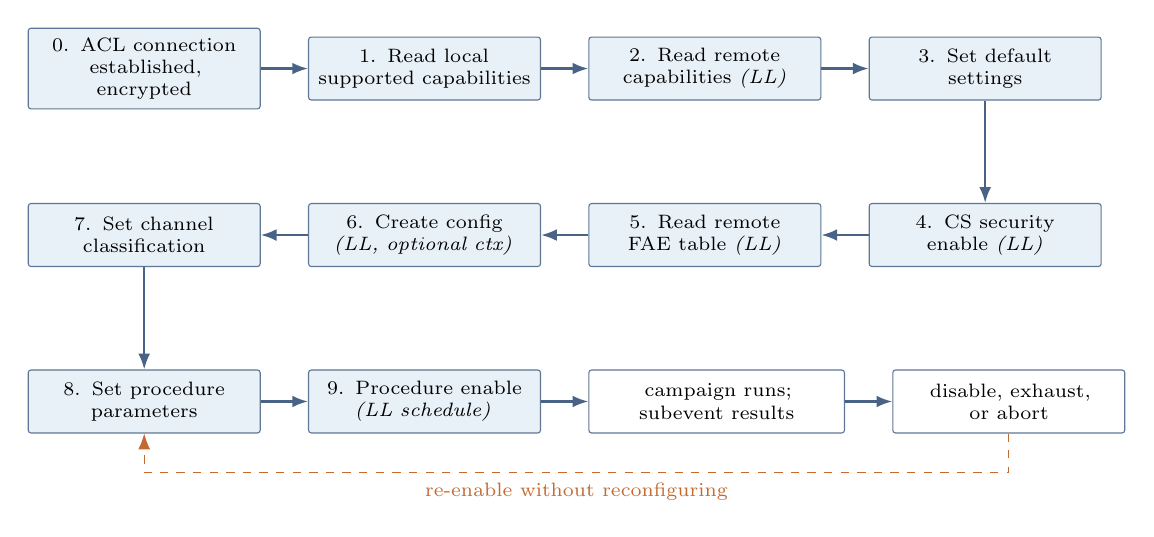
\begin{tikzpicture}[node distance=5mm and 6mm]
\node[blk,text width=27mm] (acl) {0. ACL connection\\ established, encrypted};
\node[blk,right=of acl,text width=27mm] (loccap) {1. Read local\\ supported capabilities};
\node[blk,right=of loccap,text width=27mm] (remcap) {2. Read remote\\ capabilities \emph{(LL)}};
\node[blk,right=of remcap,text width=27mm] (def) {3. Set default\\ settings};

\node[blk,below=13mm of def,text width=27mm] (sec) {4. CS security\\ enable \emph{(LL)}};
\node[blk,left=of sec,text width=27mm] (fae) {5. Read remote\\ FAE table \emph{(LL)}};
\node[blk,left=of fae,text width=27mm] (cfg) {6. Create config\\ \emph{(LL, optional ctx)}};
\node[blk,left=of cfg,text width=27mm] (cls) {7. Set channel\\ classification};

\node[blk,below=13mm of cls,text width=27mm] (par) {8. Set procedure\\ parameters};
\node[blk,right=of par,text width=27mm] (en) {9. Procedure enable\\ \emph{(LL schedule)}};
\node[pblk,right=of en,text width=30mm] (run) {campaign runs;\\ subevent results};
\node[pblk,right=of run,text width=27mm] (dis) {disable, exhaust,\\ or abort};

\draw[ar] (acl)--(loccap); \draw[ar] (loccap)--(remcap); \draw[ar] (remcap)--(def);
\draw[ar] (def.south) -- ++(0,-6.5mm) -| (sec.north);
\draw[ar] (sec)--(fae); \draw[ar] (fae)--(cfg); \draw[ar] (cfg)--(cls);
\draw[ar] (cls.south) -- ++(0,-6.5mm) -| (par.north);
\draw[ar] (par)--(en); \draw[ar] (en)--(run); \draw[ar] (run)--(dis);
\draw[dar] (dis.south) -- ++(0,-5mm) -| node[pos=0.25,below,font=\scriptsize,color=orangeacc]
   {re-enable without reconfiguring} (par.south);
\end{tikzpicture}
\caption{Configuration lifecycle. Italicised stages generate Link Layer control exchanges with the
peer. Stages 8 and 9 may be repeated for the lifetime of the configuration; stages 1--7 need not be
repeated unless capabilities, security context or configuration content change.}
\label{fig:lifecycle}
\end{figure}

\subsection{Stage 0: the ACL connection as precondition}

Channel Sounding has no connectionless form. Two devices that are not connected cannot range, and the
reason is not merely administrative: every mechanism the campaign depends on is a property of the
connection. The connection supplies a common time base with a known anchor, a reliable bidirectional
control channel for negotiating the configuration, an established security context, an agreed PHY and
data rate for that control channel, and a supervision relationship that detects loss. The connection
also supplies the identity binding: a CS result is meaningful only if it is known which peer it
describes, and the connection handle is that binding.

Encryption is the practical precondition for a secured campaign. Security establishment
(Section~\ref{sec:config-sec}) derives CS-specific material from the connection's established keys; on
an unencrypted connection it cannot proceed, and the campaign that results -- if the implementation
permits one at all -- carries randomised sequences that are not cryptographically bound to the peer,
which is precisely the condition the sounding sequence and the attack detector exist to prevent.

\subsection{Stages 1--2: capability exchange}

The local Controller reports what it can do; the remote Controller's capabilities are then fetched
across the connection with a Link Layer exchange and cached. Every subsequent parameter choice is
constrained by the intersection of the two sets. Table~\ref{tab:caps} lists the capability fields
that bear on configuration and scheduling.

\begin{table}[h]
\caption{Capability fields that constrain the campaign. Field names follow the Host interface; the
specification's table is authoritative for ranges and for fields omitted here.}
\label{tab:caps}
\centering\small
\begin{tabular}{@{}L{47mm}L{38mm}L{47mm}@{}}
\toprule
Capability & Representative range & What it constrains \\
\midrule
\code{Num\_Config\_Supported} & 1--4 & How many configurations may coexist on one connection \\
\code{Max\_Consecutive\_}\newline\code{Procedures\_Supported} & implementation & Upper bound on \code{Procedure\_Count} \\
\code{Num\_Antennas\_Supported} & 1--4 & Antenna configuration indices that are legal \\
\code{Max\_Antenna\_Paths\_Supported} & 1--4 & $\Nap$, and hence Mode-2/3 step duration \\
\code{Roles\_Supported} & initiator, reflector & Which CS role this device may take \\
\code{Optional\_Modes\_Supported} & Mode-3 & Whether Mode-3 may be a main or sub mode \\
\code{RTT\_Capability}, \code{RTT\_*\_N} & precision class and step counts & Which RTT types are usable and how many steps a precision claim needs \\
\code{Optional\_CS\_SYNC\_}\newline\code{PHYs\_Supported} & LE 2M, LE 2M 2BT & \code{CS\_SYNC\_PHY} and hence $\Tsy$ \\
\code{Optional\_Subfeatures\_}\newline\code{Supported} & companion signal, zero FAE, CSA \#3c, PBR from RTT sequence & Channel selection type; FAE handling \\
\code{T\_IP1/T\_IP2/T\_FCS/}\newline\code{T\_PM\_Times\_Supported} & bitmaps over the permitted value sets & The step timing parameters, and hence step duration \\
\code{T\_SW\_Time\_Supported} & 0, 1, 2, 4, 10\us & Antenna switch period in Mode-2/3 \\
\code{TX\_SNR\_Capability} & bitmap & Whether SNR control may be requested \\
\bottomrule
\end{tabular}
\end{table}

\begin{callout}
\textbf{Capability exchange is a scheduling input, not a formality.} $\Tsy$ follows from
\code{CS\_SYNC\_PHY}; $\Nap$ follows from the antenna capability of \emph{both} sides; $\Tip$,
$\Tipp$, $\Tsw$, $\Tpm$ and $\Tfcs$ follow from the intersection of the two supported-value bitmaps.
Every one of those appears in the step-duration equations of Section~\ref{sec:capacity}. A peer that
supports only $\Tfcs \ge 100\us$ has already reduced the number of steps that will fit in any granted
subevent, before a single scheduling parameter has been chosen.
\end{callout}

\subsection{Stage 3: default settings}

The default-settings stage is local and cheap, and it carries three things: which CS roles this
device will accept for this connection, which antenna the device will use for the \code{CS\_SYNC}
packets, and the maximum transmit power the Controller may select for CS transmissions. The last is
not merely a regulatory or power-budget control: it interacts with the reported per-step signal
quality and, through it, with the weighting used when steps are aggregated. A campaign run at a power
ceiling below the link's needs produces steps that pass their validity gates less often, which
reduces the effective aperture of every procedure.

\subsection{Stage 4: security establishment}
\label{sec:config-sec}

The CS security start procedure derives, from the connection's established security context, the
CS-specific material that personalises the campaign: an initialisation vector, an instantiation
nonce and a personalisation vector, conventionally denoted \code{CS\_IV}, \code{CS\_IN} and
\code{CS\_PV}. These seed a deterministic random bit generator whose output is consumed by the
campaign in four places.

\begin{enumerate}[leftmargin=1.5em,itemsep=2pt]
\item The 32-bit access address carried by each \code{CS\_SYNC} packet, which differs per step and is
      unpredictable to a third party.
\item The sounding sequence or random sequence payload used by the Mode-1 and Mode-3 RTT types, which
      is what makes an early-detect/late-commit attack require prediction rather than observation.
\item The channel sequence produced by the channel selection algorithm, so that the next channel is
      not predictable from the previous ones.
\item The antenna path permutation applied per step in Mode-2 and Mode-3.
\end{enumerate}

Two consequences follow for the campaign. First, security establishment must complete before a
configuration that uses a sounding or random RTT type can be enabled; the alternative is a campaign
whose sequences are not bound to the peer. Second, the derived material is a property of the
connection's security context: a re-pairing, a key refresh or a reconnection invalidates it, and the
campaign must be re-established. An implementation that caches a configuration across a reconnection
must not cache the security material with it.

\subsection{Stage 5: the FAE table}

The remote device's frequency actuation error table gives, per CS channel, the known systematic
offset between the frequency the peer intends to transmit and the frequency it actually transmits.
The Mode-0 report treats its use. At campaign level the relevant facts are that the table is fetched
once over the connection and cached, that a device declaring the zero-frequency-actuation-error
subfeature obviates the fetch, and that a stale cached table is a silent bias: it is not
re-validated during a campaign, so a peer whose calibration changes with temperature over a long
campaign will not be corrected until the table is fetched again.

\subsection{Stage 6: creating a configuration}
\label{sec:config-create}

The configuration is the content of the measurement: which modes, which RTT type, which sync PHY,
which channels, how the steps are ordered. It is not the schedule. Table~\ref{tab:createcfg} lists
the parameter set.

\begin{table}[h]
\caption{Configuration parameters. ``Negotiated'' means the value is carried to the peer in a Link
Layer configuration exchange and must be agreed; ``local'' means it applies to this device only.
Ranges are representative of the cited revision.}
\label{tab:createcfg}
\centering\small
\begin{tabular}{@{}L{40mm}L{34mm}L{20mm}L{40mm}@{}}
\toprule
Parameter & Range & Status & Effect \\
\midrule
\code{Config\_ID} & 0--3 & local & Selects one of the coexisting configurations \\
\code{Create\_Context} & local only / local and remote & local & Whether the peer is configured by this command \\
\code{Main\_Mode\_Type} & 1, 2, 3 & negotiated & The mode most steps use \\
\code{Sub\_Mode\_Type} & 1, 2, 3, none & negotiated & The interleaved secondary mode \\
\code{Min\_Main\_Mode\_Steps} & 2--255 & negotiated & Lower bound on main mode steps between sub mode steps \\
\code{Max\_Main\_Mode\_Steps} & 2--255 & negotiated & Upper bound on the same \\
\code{Main\_Mode\_Repetition} & 0--3 & negotiated & Main mode steps repeated from the previous subevent \\
\code{Mode\_0\_Steps} & 1--3 & negotiated & Mode-0 steps at the head of every subevent \\
\code{Role} & initiator / reflector & local & This device's CS role \\
\code{RTT\_Type} & AA only; 32/96-bit sounding; 32/64/96/128-bit random & negotiated & $\Tsy$, timing precision, attack resistance \\
\code{CS\_SYNC\_PHY} & LE 1M, LE 2M, LE 2M 2BT & negotiated & $\Tsy$ and receiver sensitivity \\
\code{Channel\_Map} & 10 octets, $\ge$15 channels enabled & negotiated & The frequency aperture \\
\code{Channel\_Map\_Repetition} & 1--255 & negotiated & How many times the map is traversed per procedure \\
\code{Channel\_Selection\_Type} & \#3b, \#3c & negotiated & Sequence generation \\
\code{Ch3c\_Shape}, \code{Ch3c\_Jump} & hat / X; 2--8 & negotiated & Shape parameters of CSA \#3c \\
\bottomrule
\end{tabular}
\end{table}

\subsubsection{Legal main/sub mode combinations}

Not every pair is permitted. The rule follows from what a sub mode is for: it supplies the
complementary observable to the main mode, so that a procedure yields both an unambiguous coarse
range and a precise ambiguous one.

\begin{table}[h]
\caption{Permitted main and sub mode combinations, and what each yields.}
\label{tab:modecombo}
\centering\small
\begin{tabular}{@{}L{22mm}L{22mm}L{40mm}L{48mm}@{}}
\toprule
Main mode & Sub mode & Observables per procedure & Typical intent \\
\midrule
Mode-1 & none   & RTT only & Coarse ranging; presence and integrity \\
Mode-1 & Mode-2 & RTT dense, PBR sparse & RTT-led, PBR used to refine \\
Mode-2 & none   & PBR only & Precise but ambiguous; needs external disambiguation \\
Mode-2 & Mode-1 & PBR dense, RTT sparse & The common high-accuracy configuration \\
Mode-2 & Mode-3 & PBR dense, combined sparse & PBR-led with combined anchors \\
Mode-3 & none   & RTT and PBR every step & Maximum information per step, longest step \\
Mode-3 & Mode-2 & Combined dense, PBR sparse & Mode-3 led, cheaper interleaved steps \\
\bottomrule
\end{tabular}
\end{table}

\begin{callout}
\textbf{Mode-0 is not a main or sub mode.} It is not selected by \code{Main\_Mode\_Type} or
\code{Sub\_Mode\_Type}, and it is not optional. It is inserted at the head of every subevent by the
scheduling rules, in the quantity given by \code{Mode\_0\_Steps}. This is a structural statement about
the campaign, not a per-step one: the frequency reference is a \emph{subevent} property, and the cost
of establishing it is paid once per subevent, not once per procedure.
\end{callout}

\subsection{Stage 7: channel classification}

Channel classification is the mechanism by which a device tells the campaign which CS channels it
believes are unusable. It is distinct from the ACL connection's own channel map, and distinct from
the configuration's \code{Channel\_Map}: the configuration states which channels the campaign may
use, and classification states which of them are currently believed bad. Section~\ref{sec:channels}
develops the interaction, including the important asymmetry that classification updates take effect
at a procedure boundary rather than immediately.

\subsection{Stage 8: procedure parameters}
\label{sec:config-procparams}

This is where the Host expresses the schedule it wants. Every scheduling quantity here except the
antenna configuration is a bound rather than a value.

\begin{table}[h]
\caption{Procedure parameters. Note that six of the thirteen are minimum/maximum pairs: they express
an acceptable range, not a request for a specific schedule.}
\label{tab:procparams}
\centering\small
\begin{tabular}{@{}L{42mm}L{34mm}L{18mm}L{40mm}@{}}
\toprule
Parameter & Range and units & Kind & Effect \\
\midrule
\code{Max\_Procedure\_Len} & 1--65535 $\times$ 0.625\,ms (to 40.96\,s) & bound & Upper limit on one procedure's duration \\
\code{Min\_Procedure\_Interval} & 1--65535 connection intervals & bound & Fastest acceptable repetition \\
\code{Max\_Procedure\_Interval} & 1--65535 connection intervals & bound & Slowest acceptable repetition \\
\code{Max\_Procedure\_Count} & 1--65535; 0 for continuous & bound & Campaign length \\
\code{Min\_Subevent\_Len} & 1250--3\,999\,999\us & bound & Smallest acceptable coherent block \\
\code{Max\_Subevent\_Len} & 1250--3\,999\,999\us & bound & Largest acceptable coherent block \\
\code{Tone\_Antenna\_}\newline\code{Config\_Selection} & 0--7 & value & $\Nap$, and Mode-2/3 step duration \\
\code{PHY} & LE 1M / 2M / Coded & value & PHY used for the procedure's LL signalling \\
\code{Tx\_Power\_Delta} & dB, or ``no recommendation'' & value & Requested deviation from the link's power \\
\code{Preferred\_Peer\_Antenna} & bitmap over 4 elements & value & Which peer elements to use \\
\code{SNR\_Control\_Initiator} & 18/21/24/27/30\,dB or off & value & Transmit power control target at the initiator \\
\code{SNR\_Control\_Reflector} & as above & value & The same at the reflector \\
\bottomrule
\end{tabular}
\end{table}

\subsection{Stage 9: enable, and the schedule that comes back}
\label{sec:config-enable}

Enabling the procedure is the point at which the abstraction inverts. Up to here the Host has been
supplying constraints; from here the Controller supplies facts. The completion event reports the
settled schedule, and it is the authoritative description of what will happen on air.

\begin{table}[h]
\caption{The settled schedule reported at procedure enable. Every field is an answer, not a request.}
\label{tab:enablecomplete}
\centering\small
\begin{tabular}{@{}L{38mm}L{28mm}L{68mm}@{}}
\toprule
Reported field & Units & Interpretation \\
\midrule
\code{Selected\_TX\_Power} & dBm & The power the Controller will actually use \\
\code{Subevent\_Len} & \ensuremath{\upmu}s & Granted subevent length; the coherence block \\
\code{Subevents\_Per\_Event} & count (to 16) & Subevents packed into one CS event \\
\code{Subevent\_Interval} & 625\us; 0 if one subevent & Start-to-start spacing within an event \\
\code{Event\_Interval} & connection intervals & Spacing of CS event anchors \\
\code{Procedure\_Interval} & connection intervals & Spacing of procedure anchors \\
\code{Procedure\_Count} & count; 0 for continuous & Campaign length as settled \\
\code{Max\_Procedure\_Len} & 0.625\,ms & The granted procedure length bound \\
\bottomrule
\end{tabular}
\end{table}

\begin{callout}
\textbf{Read the reply, then compute.} Measurement rate, radio duty cycle, energy per fix, coherence
structure and channel coverage per procedure are all functions of the fields in
Table~\ref{tab:enablecomplete} and of the per-mode step durations -- not of the ranges requested in
Table~\ref{tab:procparams}. Section~\ref{sec:worked} performs that computation end to end for a
representative configuration.
\end{callout}

% ============================================================
\section{The ACL connection as substrate}
\label{sec:acl}
% ============================================================

The ACL connection is not merely a prerequisite that can be satisfied and then forgotten. It enters
the campaign continuously and in four distinct capacities. This section takes them in turn and closes
with a summary table mapping each ACL parameter to the CS quantity it controls.

\subsection{Capacity one: the time base}
\label{sec:acl-timebase}

A CS procedure starts at a stated offset from the anchor point of a stated ACL connection event. This
single sentence carries most of the coupling.

The ACL connection defines a periodic sequence of anchor points separated by the connection interval
$\Tconn$, numbered by a connection event counter that both devices maintain and that survives
peripheral latency and missed events. Because both Controllers already agree on that sequence to
within the accuracy required to maintain the link, it is the natural common clock, and Channel
Sounding uses it as such: the campaign is expressed as \emph{(connection event number, offset)} pairs
rather than as absolute times. No new synchronisation mechanism is introduced at campaign level; the
sub-microsecond alignment that ranging needs is established inside each subevent by the Mode-0 steps,
on top of the coarse alignment the connection already provides.

\begin{figure}[h]
\centering
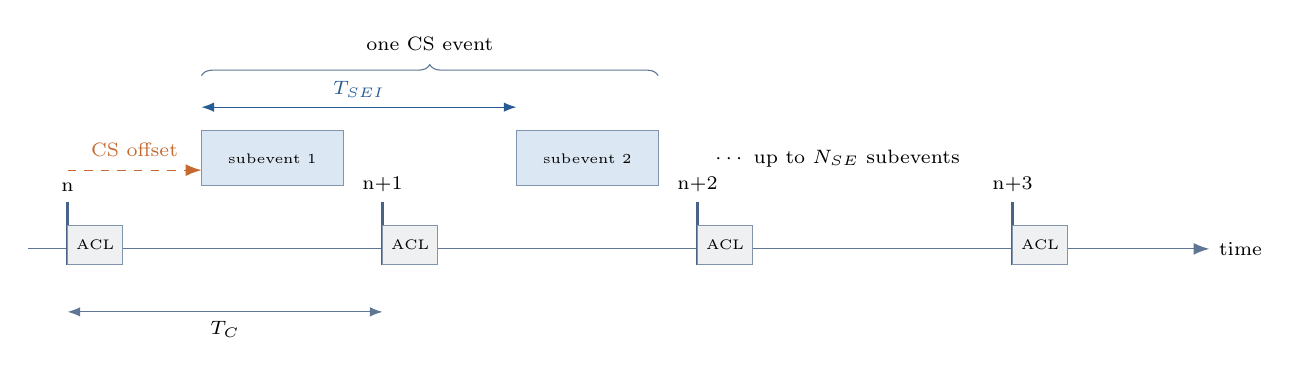
\begin{tikzpicture}[x=1mm,y=1mm]
% ACL anchor timeline
\draw[-{Latex[length=2mm]},draw=navy!70] (0,0) -- (150,0) node[right,font=\scriptsize] {time};
\foreach \x/\n in {5/n, 45/n+1, 85/n+2, 125/n+3}{
  \draw[draw=navy!80,thick] (\x,-2) -- (\x,6);
  \node[font=\scriptsize,anchor=south] at (\x,6) {\n};
  \draw[slot,fill=greybox] (\x,-2) rectangle (\x+7,3) node[midway,font=\tiny] {ACL};
}
\draw[{Latex[length=1.6mm]}-{Latex[length=1.6mm]},draw=navy!70] (5,-8) -- (45,-8)
  node[midway,below,font=\scriptsize] {$\Tconn$};

% CS offset and subevents
\draw[dar] (5,10) -- (22,10);
\node[font=\scriptsize,color=orangeacc,anchor=south] at (13.5,10.5) {CS offset};
\draw[slot,fill=boxblue] (22,8) rectangle (40,15) node[midway,font=\tiny] {subevent 1};
\draw[slot,fill=boxblue] (62,8) rectangle (80,15) node[midway,font=\tiny] {subevent 2};
\draw[{Latex[length=1.6mm]}-{Latex[length=1.6mm]},draw=accent] (22,18) -- (62,18)
  node[midway,above,font=\scriptsize,color=accent] {$\Tsei$};
\node[font=\scriptsize,anchor=west] at (86,11.5) {$\cdots$ up to $\Nse$ subevents};

\draw[decorate,decoration={brace,amplitude=4pt},draw=navy!70] (22,22) -- (80,22);
\node[font=\scriptsize,anchor=south] at (51,24) {one CS event};
\end{tikzpicture}
\caption{Anchoring. The CS event begins at a fixed offset from the ACL connection event anchor point
of a nominated connection event, and its subevents are spaced by $\Tsei$. The ACL connection event
itself continues to occur; CS activity is placed around it, not instead of it.}
\label{fig:anchor}
\end{figure}

Three consequences deserve to be stated explicitly.

\emph{The connection interval is the scheduling quantum.} The spacing between CS events and between
CS procedures is expressed in whole connection intervals. A campaign on a 7.5\,ms connection can be
repeated at 7.5\,ms granularity; the same campaign on a 100\,ms connection can only be repeated at
100\,ms granularity. A Host that wants a 250\,ms update rate on a 100\,ms connection cannot have it:
it can have 200\,ms or 300\,ms.

\emph{The connection interval bounds the subevent.} CS activity must coexist with the connection
events themselves and with whatever else the Controller has scheduled. A subevent whose length
approaches the connection interval leaves no room, and the Controller will grant less than was asked
for -- which, as Section~\ref{sec:hier-coherence} shows, silently changes the coherence structure of
the measurement by splitting what the Host expected to be one subevent into several.

\emph{Anchor drift is common-mode.} Because both devices track the same connection event counter and
the same anchor sequence, slow drift of the pair's shared timing relative to absolute time does not
disturb the campaign. What would disturb it is a change in the anchor sequence itself, which is the
subject of Section~\ref{sec:acl-updates}.

\subsection{Capacity two: the counting unit and interval arithmetic}

Given the settled schedule, the campaign's timing is fully determined:

\begin{align}
\text{CS event period} \;&=\; \Nei \,\Tconn, \label{eq:eventperiod}\\
\text{CS procedure period} \;&=\; \Npi \,\Tconn, \label{eq:procperiod}\\
\text{subevent starts within an event} \;&=\; \{0,\ \Tsei,\ 2\Tsei,\ \dots,\ (\Nse-1)\Tsei\},
   \label{eq:sestarts}\\
\text{campaign duration} \;&=\; \Npc \,\Npi \,\Tconn \quad (\Npc \ne 0).
   \label{eq:campaignlen}
\end{align}

Two structural constraints link these. First, a procedure must be able to contain the events it
needs: the number of CS events in a procedure is bounded by $\lceil \Npi / \Nei \rceil$, and if the
procedure's step budget requires more events than that, the procedure is truncated rather than
extended. Second, the granted $\Tpl$ bounds the procedure independently of the event structure; a
procedure ends when it has executed its steps, when it reaches $\Tpl$, or when it is aborted,
whichever comes first.

\begin{callout}
\textbf{$\Nei = 1$ is not always available.} An implementation may be unable to place CS events on
every connection event -- because the CS event plus the connection event plus scheduling margin does
not fit in $\Tconn$, or because other links share the radio. Controllers commonly return $\Nei = 2$
where the Host asked for the fastest possible schedule. This is legitimate: the Host asked for a
range, and the Controller answered within it. The observable effect is that the measurement rate is
half what a naive calculation predicted, and the only reliable way to know is to read
$\Nei$ back from the enable completion.
\end{callout}

\subsection{Capacity three: the security context}

Section~\ref{sec:config-sec} described the derivation. The campaign-level point is the coupling in the
other direction: anything that disturbs the connection's security context disturbs the campaign.
Re-pairing, an encryption pause and restart, or a key refresh invalidate the CS material, and a
correct implementation re-runs security establishment rather than continuing with stale nonce
material. Continuing with stale material is not a subtle degradation -- it means the access addresses
and sequences of the new campaign are predictable from observation of the old one, which is the exact
capability a distance-reduction attacker needs.

\subsection{Capacity four: liveness, latency and updates}
\label{sec:acl-updates}

\subsubsection{Peripheral latency}

Peripheral latency permits the Peripheral to skip connection events. The anchor sequence is
unaffected -- the counter still advances -- so the arithmetic of
Equations~\eqref{eq:eventperiod}--\eqref{eq:campaignlen} still holds. What changes is the practical
one: a Peripheral that is skipping connection events to save power must nonetheless wake for the
connection events that anchor CS events. A campaign therefore erodes the power saving that latency
was configured to provide, and a Host that measures the energy cost of ranging must attribute the
extra wake-ups to the campaign, not to the link.

\subsubsection{Connection parameter updates}

A connection parameter update changes $\Tconn$, and therefore changes the physical meaning of every
interval expressed in connection intervals. A campaign configured for a 250\,ms procedure period as
$\Npi = 5$ on a 50\,ms connection becomes a 100\,ms procedure period if the connection interval is
changed to 20\,ms, without any CS parameter changing. Two disciplines follow: an application that
depends on a particular update rate must re-read its own schedule after any connection parameter
update, and a Host that intends to change connection parameters during a campaign should expect the
Controller to disable, re-negotiate or reject rather than silently re-time.

\subsubsection{Subrating}

Connection subrating multiplies the effective connection interval for data purposes while preserving
the underlying anchor sequence. Where it is in use, the relationship between the connection interval
the Host configured and the anchor points actually available for CS anchoring is no longer the naive
one, and the settled $\Nei$ must again be read rather than assumed.

\subsubsection{Supervision timeout and termination}

The campaign is subordinate to the connection. Loss of the connection terminates the campaign
immediately and without a procedure completion; the Host observes a disconnection, not a CS event.
The supervision timeout therefore sets the worst-case time for which a ranging application may
continue to believe a campaign is running after the peer has in fact gone. Applications that gate
physical access on proximity should treat the supervision timeout, not the procedure interval, as the
staleness bound on the last result.

\subsection{The scheduling negotiation itself}
\label{sec:acl-negotiation}

The Link Layer carries a small family of CS control procedures over the ACL connection. Their names
follow the usual \code{LL\_CS\_*} pattern and their functions divide cleanly:

\begin{table}[h]
\caption{Link Layer control exchanges used by the campaign, and what each carries. PDU names follow
the cited revision.}
\label{tab:llcp}
\centering\small
\begin{tabular}{@{}L{44mm}L{40mm}L{52mm}@{}}
\toprule
Exchange & Stage & Carries \\
\midrule
\code{LL\_CS\_CAPABILITIES\_REQ/RSP} & 2 & The capability set of Table~\ref{tab:caps} \\
\code{LL\_CS\_SEC\_REQ/RSP} & 4 & Material for deriving \code{CS\_IV}, \code{CS\_IN}, \code{CS\_PV} \\
\code{LL\_CS\_FAE\_REQ/RSP} & 5 & The per-channel frequency actuation error table \\
\code{LL\_CS\_CONFIG\_REQ/RSP} & 6 & The configuration content of Table~\ref{tab:createcfg} \\
\code{LL\_CS\_CHANNEL\_MAP\_IND} & 7 & Updated channel classification \\
\code{LL\_CS\_REQ / RSP / IND} & 9 & The concrete schedule: anchor connection event, offset,
                                     subevent length and interval, event and procedure intervals \\
\code{LL\_CS\_TERMINATE\_IND} & any & Orderly termination of a running campaign \\
\bottomrule
\end{tabular}
\end{table}

The third row from the bottom is the one that answers the question of who decides the schedule. The
initiator's Controller composes a proposal from its Host's requested ranges, its own scheduling
constraints and the peer's declared capabilities, and offers it -- typically as a set of acceptable
offsets rather than a single instant, so the reflector has room to fit the campaign around its own
commitments. The reflector's Controller selects within what was offered and replies; the initiator
confirms. Only then do both Controllers report the settled schedule to their respective Hosts.

\begin{callout}
\textbf{Why a reflector Host cannot dictate the rate.} The reflector's procedure parameters constrain
what it will accept, and a proposal outside them is refused -- which manifests as a failed enable, not
as a slower campaign. A reflector that wants a faster campaign must either widen its acceptable range
so that a proposal can succeed, or influence the initiator through the application layer. This is a
frequent source of confusion when both sides are developed independently and each assumes its own
requested interval is the operating one.
\end{callout}

\subsection{Summary: ACL parameter to CS effect}

\begin{table}[htb]
\caption{How each parameter of the ACL connection enters the campaign. The right-hand column names
the mechanism, not merely the correlation.}
\label{tab:aclmap}
\centering\small
\begin{tabular}{@{}L{34mm}L{50mm}L{52mm}@{}}
\toprule
ACL parameter & Enters the campaign as & Mechanism \\
\midrule
Connection interval $\Tconn$
  & The scheduling quantum for $\Nei$ and $\Npi$; the space available for a subevent
  & Equations~\eqref{eq:eventperiod}--\eqref{eq:campaignlen}; subevent must fit between connection
    events \\
Connection event counter
  & The shared timeline on which the campaign is expressed
  & Procedure start is (event number, offset) \\
Connection event anchor point
  & The origin of the CS offset
  & Figure~\ref{fig:anchor} \\
Peripheral latency
  & Wake-up obligations that the campaign reinstates
  & CS events anchor to connection events that latency would otherwise skip \\
Supervision timeout
  & Worst-case staleness bound on the last result
  & Campaign ends silently with the connection \\
Encryption and key material
  & The root of \code{CS\_IV}, \code{CS\_IN}, \code{CS\_PV}
  & Security establishment, Section~\ref{sec:config-sec} \\
Connection PHY
  & The rate of the control exchanges, hence configuration latency
  & Stages 2, 4, 5, 6, 9 are LL round trips \\
Connection subrating
  & Alters which anchors are practically available
  & $\Nei$ granted by the Controller \\
ACL channel map
  & Independent of the CS channel map, but a proxy for the same interference
  & Classification input, Section~\ref{sec:channels} \\
Connection handle
  & Identity binding of every CS result
  & All CS commands and events are per handle \\
\bottomrule
\end{tabular}
\end{table}

% ============================================================
\section{The scheduling hierarchy}
\label{sec:hier}
% ============================================================

\subsection{The whole structure in one picture}

Figure~\ref{fig:hierarchy} shows the five levels on one time axis, with each level expanded from the
one above. The figure is the reference for the rest of the report: every scheduling parameter names
one of its dimensions.

\begin{figure}[h]
\centering
\resizebox{\textwidth}{!}{%
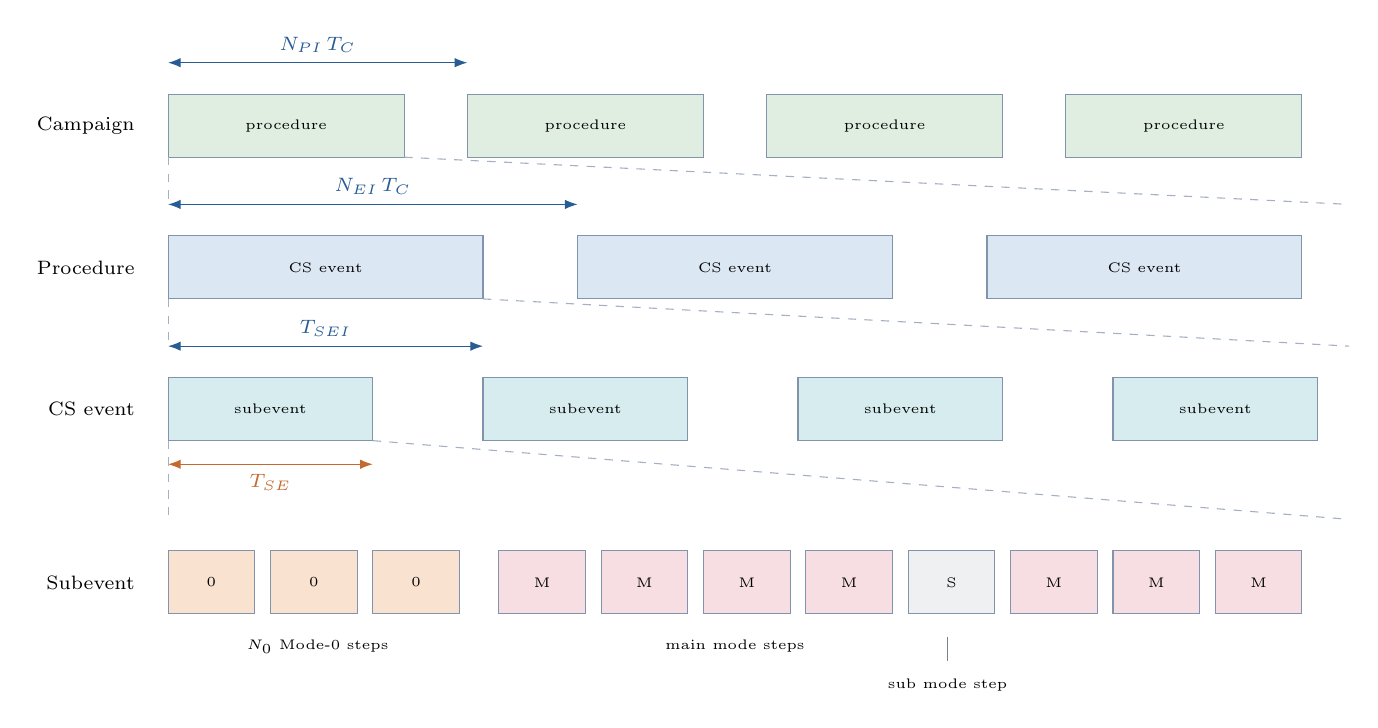
\begin{tikzpicture}[x=1mm,y=1mm]
% ---------- level 1: campaign ----------
\node[font=\scriptsize,anchor=east] at (-3,44) {Campaign};
\foreach \x in {0,38,76,114}{
  \draw[slot,fill=greenbox] (\x,40) rectangle (\x+30,48) node[midway,font=\tiny] {procedure};
}
\draw[{Latex[length=1.6mm]}-{Latex[length=1.6mm]},draw=accent] (0,52) -- (38,52)
  node[midway,above,font=\scriptsize,color=accent] {$\Npi\,\Tconn$};

% ---------- level 2: procedure -> events ----------
\node[font=\scriptsize,anchor=east] at (-3,26) {Procedure};
\draw[draw=navy!40,dashed] (0,40) -- (0,34);
\draw[draw=navy!40,dashed] (30,40) -- (150,34);
\foreach \x in {0,52,104}{
  \draw[slot,fill=boxblue] (\x,22) rectangle (\x+40,30) node[midway,font=\tiny] {CS event};
}
\draw[{Latex[length=1.6mm]}-{Latex[length=1.6mm]},draw=accent] (0,34) -- (52,34)
  node[midway,above,font=\scriptsize,color=accent] {$\Nei\,\Tconn$};

% ---------- level 3: event -> subevents ----------
\node[font=\scriptsize,anchor=east] at (-3,8) {CS event};
\draw[draw=navy!40,dashed] (0,22) -- (0,16);
\draw[draw=navy!40,dashed] (40,22) -- (150,16);
\foreach \x in {0,40,80,120}{
  \draw[slot,fill=tealbox] (\x,4) rectangle (\x+26,12) node[midway,font=\tiny] {subevent};
}
\draw[{Latex[length=1.6mm]}-{Latex[length=1.6mm]},draw=accent] (0,16) -- (40,16)
  node[midway,above,font=\scriptsize,color=accent] {$\Tsei$};
\draw[{Latex[length=1.6mm]}-{Latex[length=1.6mm]},draw=orangeacc] (0,1) -- (26,1)
  node[midway,below,font=\scriptsize,color=orangeacc] {$\Tse$};

% ---------- level 4: subevent -> steps ----------
\node[font=\scriptsize,anchor=east] at (-3,-14) {Subevent};
\draw[draw=navy!40,dashed] (0,4) -- (0,-6);
\draw[draw=navy!40,dashed] (26,4) -- (150,-6);
\foreach \x/\lab/\col in {0/0/peachbox, 13/0/peachbox, 26/0/peachbox,
                          42/M/pinkbox, 55/M/pinkbox, 68/M/pinkbox, 81/M/pinkbox,
                          94/S/greybox, 107/M/pinkbox, 120/M/pinkbox, 133/M/pinkbox}{
  \draw[slot,fill=\col] (\x,-18) rectangle (\x+11,-10) node[midway,font=\tiny] {\lab};
}
\node[font=\tiny,anchor=north,align=center] at (19,-20) {$N_0$ Mode-0 steps};
\node[font=\tiny,anchor=north,align=center] at (72,-20) {main mode steps};
\node[font=\tiny,anchor=north,align=center] at (99,-25) {sub mode step};
\draw[draw=rulegrey,thin] (99,-21) -- (99,-24);
\end{tikzpicture}}
\vspace{6mm}
\caption{The campaign hierarchy on one axis. Each level is an expansion of one box of the level
above. M denotes a main mode step, S a sub mode step, 0 a Mode-0 step. Widths are illustrative; the
per-mode step durations of Section~\ref{sec:capacity} differ substantially between modes.}
\label{fig:hierarchy}
\end{figure}

\subsection{The step}

The step is the atom. It occupies one channel, uses one mode, and consists of a reciprocal exchange
whose structure is given in the companion reports. Between consecutive scheduled steps the radio must
retune, and the frequency-change period $\Tfcs$ is reserved for that purpose. $\Tfcs$ is a
configuration-negotiated value drawn from a permitted set (representatively 15, 20, 30, 40, 50, 60,
80, 100, 120 and 150\us) and it is not measurement time: it is pure overhead that scales with the
step count, and at the fast end of the range it is a small fraction of a step while at the slow end it
can approach half of a Mode-1 step.

\subsection{The subevent}
\label{sec:hier-coherence}

The subevent is the coherence block, and it is the most consequential level of the hierarchy for
estimation quality.

A subevent begins with $N_0 \in \{1,2,3\}$ Mode-0 steps, whose combined result is the subevent
frequency reference $\FFO^{*}_{RX}$. Every subsequent step in that subevent is processed against that
reference. Steps in a different subevent are processed against a different reference, estimated at a
different time from different noise. Two practical rules follow.

\emph{Phase measurements do not cross subevent boundaries for free.} A Mode-2 phase-slope fit run
across channels drawn from two subevents inherits the difference between the two frequency references
as an additional term. That term is small when the references are good, but it is not zero, and it is
not modelled by a fit that assumes one common reference. Where the highest accuracy is required, the
per-subevent fits should be formed first and combined afterwards, or the configuration should be
arranged so that a procedure's PBR steps fall in a single subevent.

\emph{Requesting a long subevent is requesting coherence, not just capacity.} The Host's
\code{Min\_Subevent\_Len} is the mechanism by which it says ``do not split my measurement''. If the
Controller cannot grant it, the enable either fails or returns a shorter subevent -- and a shorter
subevent means more subevents, more Mode-0 overhead, and a fragmented coherence structure.

The subevent also carries a fixed cost. The $N_0$ Mode-0 steps are the longest steps in the campaign
(Section~\ref{sec:capacity}), and they measure no distance. The Mode-0 overhead fraction is

\begin{equation}
\eta_0 \;=\; \frac{N_0\,(T_{step,0} + \Tfcs)}{\Tse},
\label{eq:mode0overhead}
\end{equation}

which for a short subevent can exceed a fifth of the available time. Choosing $N_0 = 3$ for
robustness and then requesting a short subevent is a self-defeating combination.

\subsection{The event}

The event is the scheduling container that binds subevents to one ACL anchor. Its parameters are
$\Nse$, the number of subevents it holds, and $\Tsei$, their spacing. Where $\Nse = 1$ the subevent
interval is meaningless and is reported as zero.

The event exists because the useful measurement block and the connection's natural rhythm are
different sizes. A single subevent of a few hundred microseconds is far shorter than a 50\,ms
connection interval; packing several subevents into one event lets the campaign use the interval
efficiently without demanding a CS event at every connection event. Conversely, where the connection
interval is short, $\Nse = 1$ and $\Nei > 1$ is the natural arrangement.

\begin{callout}
\textbf{Subevent interval is quantised to 625\us.} Like several other LE scheduling quantities,
$\Tsei$ is counted in 625\us units. A Controller cannot place subevents 400\us apart, so a subevent
that is granted 300\us of length still occupies a 625\us cadence slot when $\Nse > 1$. The gap is
real idle time and should be counted as such in energy models.
\end{callout}

\subsection{The procedure}

The procedure is the natural unit of a ranging result. Its content is defined by the channel
sequence: a procedure traverses the enabled channels of the configuration's channel map, repeated
\code{Channel\_Map\_Repetition} times, in the order produced by the selected channel selection
algorithm. When the sequence is exhausted the procedure ends.

Three bounds can end a procedure before its sequence is exhausted:

\begin{enumerate}[leftmargin=1.5em,itemsep=2pt]
\item the granted $\Tpl$, in 0.625\,ms units, elapses;
\item the events available before the next procedure anchor, $\lceil \Npi/\Nei \rceil$, are used up;
\item an abort condition arises (Section~\ref{sec:results-abort}).
\end{enumerate}

A truncated procedure is not an error and is reported as such, but it changes the frequency aperture
of that result, and an aggregation layer that weights procedures equally without checking their
completion status will produce inconsistent precision from one fix to the next.

\subsection{The campaign}

Finally, \code{Procedure\_Count} sets how many procedures the enable authorises: a finite count for a
bounded burst, or the continuous setting for a campaign that runs until explicitly disabled. Three
patterns are common in practice.

\begin{table}[h]
\caption{Common campaign patterns and their parameter shapes.}
\label{tab:patterns}
\centering\small
\begin{tabular}{@{}L{32mm}L{40mm}L{28mm}L{34mm}@{}}
\toprule
Pattern & Intent & $\Npc$ & $\Npi$ \\
\midrule
Single shot & One distance, minimum energy & 1 & irrelevant \\
Burst & Average several procedures into one fix & 4--16 & smallest granted \\
Continuous tracking & Maintain a distance estimate & continuous & set by required update rate \\
Duty-cycled tracking & Presence with occasional refinement & continuous & large; widen with range \\
\bottomrule
\end{tabular}
\end{table}

% ============================================================
\section{Step composition inside a subevent}
\label{sec:steps}
% ============================================================

This section answers the third question of Section~\ref{sec:scope}: given a configuration, in what
order do steps of the different modes actually occur?

\subsection{The ordering rule}

The ordering is fixed by three rules applied in sequence.

\begin{enumerate}[leftmargin=1.6em,itemsep=3pt]
\item \textbf{Mode-0 first.} Every subevent begins with exactly $N_0$ Mode-0 steps, where
      $N_0 = $ \code{Mode\_0\_Steps} $\in \{1,2,3\}$. They are not optional, they are not distributed
      through the subevent, and they are repeated in every subevent of the procedure -- not once per
      procedure.
\item \textbf{Repetition of the previous subevent's main mode steps.} The next $R_m = $
      \code{Main\_Mode\_Repetition} steps repeat main mode steps from the end of the preceding
      subevent, on the same channels. For the first subevent of a procedure there is nothing to
      repeat and the rule is inert. $R_m \in \{0,1,2,3\}$.
\item \textbf{Main mode steps with sub mode steps interleaved.} The remainder of the subevent is
      filled with main mode steps, into which sub mode steps are inserted such that the number of
      consecutive main mode steps between two sub mode steps lies in
      $[n_{\min}, n_{\max}] = [$\code{Min\_Main\_Mode\_Steps}, \code{Max\_Main\_Mode\_Steps}$]$. The
      exact cadence within that range is the Controller's choice, and it need not be constant. Where
      no sub mode is configured, the remainder is main mode steps only.
\end{enumerate}

\begin{figure}[h]
\centering
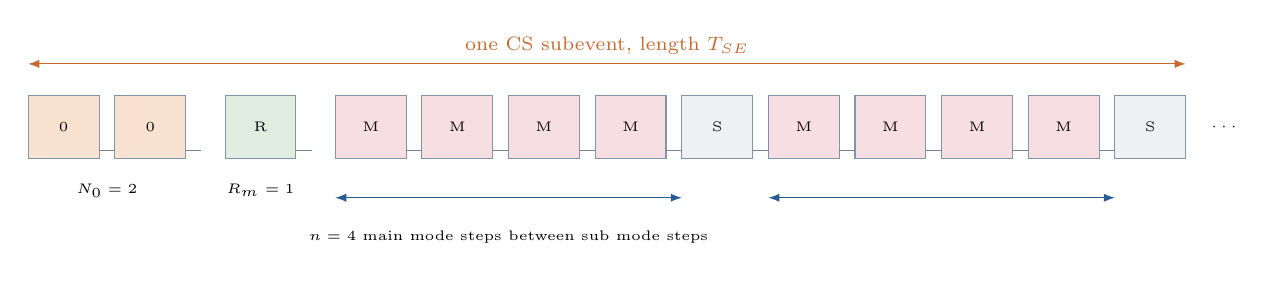
\begin{tikzpicture}[x=1mm,y=1mm]
\foreach \x/\lab/\col in {0/0/peachbox, 11/0/peachbox,
                          25/R/greenbox,
                          39/M/pinkbox, 50/M/pinkbox, 61/M/pinkbox, 72/M/pinkbox,
                          83/S/greybox,
                          94/M/pinkbox, 105/M/pinkbox, 116/M/pinkbox, 127/M/pinkbox,
                          138/S/greybox}{
  \draw[slot,fill=\col] (\x,0) rectangle (\x+9,8) node[midway,font=\tiny] {\lab};
}
\foreach \x in {9,20,34,48,59,70,81,92,103,114,125,136}{
  \draw[draw=rulegrey,thin] (\x,1) -- (\x+2,1);
}
\node[font=\tiny,anchor=north] at (10,-2) {$N_0=2$};
\node[font=\tiny,anchor=north] at (29.5,-2) {$R_m=1$};
\node[font=\tiny,anchor=north] at (61,-8) {$n=4$ main mode steps between sub mode steps};
\draw[{Latex[length=1.4mm]}-{Latex[length=1.4mm]},draw=accent] (39,-5) -- (83,-5);
\draw[{Latex[length=1.4mm]}-{Latex[length=1.4mm]},draw=accent] (94,-5) -- (138,-5);
\node[font=\tiny,anchor=west] at (149,4) {$\cdots$};
\draw[{Latex[length=1.4mm]}-{Latex[length=1.4mm]},draw=orangeacc] (0,12) -- (147,12)
   node[midway,above,font=\scriptsize,color=orangeacc] {one CS subevent, length $\Tse$};
\end{tikzpicture}
\vspace{4mm}
\caption{Step ordering inside a subevent for $N_0 = 2$, $R_m = 1$, sub mode configured, and a
Controller-chosen cadence of $n = 4$. The short grey marks between steps are the frequency-change
periods $\Tfcs$. R denotes a repeated main mode step from the previous subevent.}
\label{fig:ordering}
\end{figure}

\subsection{What each rule is for}

\subsubsection{Why Mode-0 is per subevent}

The Mode-0 result is a frequency reference with a finite useful life. Crystal offsets drift with
temperature and supply, and the ranging chain's tolerance for residual frequency error is tight: the
Mode-2 report shows that a residual offset multiplied by the reciprocal measurement interval reads
directly as distance. Re-establishing the reference at the head of each coherence block bounds the
age of the reference to at most one subevent, which is the same bound that makes the subevent a valid
coherence block in the first place. The choice of $N_0$ trades that robustness against
Equation~\eqref{eq:mode0overhead}: $N_0 = 1$ gives one frequency estimate with no redundancy and no
means of detecting a bad one; $N_0 = 3$ permits a median or a validity-gated average at a cost that
Section~\ref{sec:capacity} quantifies.

\subsubsection{Why main mode steps are repeated across the boundary}

$R_m$ exists to create deliberate overlap. The repeated steps measure the same channels in two
consecutive subevents, and therefore under two different frequency references. Their difference is a
direct observation of the inter-subevent reference discontinuity discussed in
Section~\ref{sec:hier-coherence}, and it is what allows measurements from adjacent subevents to be
stitched into one aperture rather than merely averaged. $R_m = 0$ is the cheapest and is appropriate
when a procedure fits in one subevent; $R_m \ge 1$ is what makes a multi-subevent procedure
coherently combinable.

The cost is exact and easy to overlook: $R_m$ steps per subevent are spent re-measuring channels
already measured, so they do not extend the frequency aperture. In a procedure of $S$ subevents the
campaign spends $R_m(S-1)$ steps on continuity.

\subsubsection{Why sub mode steps are interleaved rather than blocked}

A sub mode exists to supply the complementary observable, and the complementary observable is only
useful if it is contemporaneous with the main one. A block of RTT steps at the end of a procedure
would be separated from the early PBR steps by the whole procedure length, during which the target
may have moved. Interleaving at a cadence of $n_{\min}$ to $n_{\max}$ main steps distributes the
disambiguating measurement through the aperture, so that the coarse and fine observables describe the
same instant to within a few steps.

The cadence is a direct trade. Table~\ref{tab:cadence} gives the arithmetic.

\begin{table}[h]
\caption{Sub mode cadence. The fraction of steps spent on the sub mode is $1/(n+1)$ for a constant
cadence of $n$ main mode steps per sub mode step.}
\label{tab:cadence}
\centering\small
\begin{tabular}{@{}rrrL{70mm}@{}}
\toprule
$n$ & Sub mode fraction & Main mode fraction & Character \\
\midrule
2  & 33.3\,\% & 66.7\,\% & Sub mode heavily sampled; large capacity cost \\
4  & 20.0\,\% & 80.0\,\% & Robust disambiguation; common choice \\
9  & 10.0\,\% & 90.0\,\% & Aperture-favouring; adequate where ambiguity is small \\
19 & 5.0\,\%  & 95.0\,\% & Minimal disambiguation; assumes prior range knowledge \\
\bottomrule
\end{tabular}
\end{table}

\begin{callout}
\textbf{$n_{\min}$ and $n_{\max}$ are a range given to the Controller, not a schedule.} A Host that
needs a known number of sub mode steps per procedure should set $n_{\min} = n_{\max}$ and accept the
scheduling rigidity, or -- better -- count the reported step modes in the subevent results rather
than predicting them. The results report the mode of every step, so the realised cadence is always
observable after the fact.
\end{callout}

\subsection{Channel assignment}

Each step occupies one channel. The channels are consumed in the order given by the sequence that the
selected channel selection algorithm generates for the procedure from the enabled channel map and the
campaign's random material, with two structural exceptions: the Mode-0 steps at the head of a
subevent take their channels from the head of that subevent's allocation, and the $R_m$ repeated
steps deliberately re-use the channels of the steps they repeat.

The consequence for aperture planning is that the number of \emph{distinct} channels a procedure
measures is not the number of steps it executes. For a procedure of $S$ subevents:

\begin{equation}
N_{\text{distinct}} \;\le\; \underbrace{S\,\Nst}_{\text{steps executed}}
   \;-\; \underbrace{S\,N_0}_{\text{Mode-0}}
   \;-\; \underbrace{R_m (S-1)}_{\text{repetition}},
\label{eq:distinct}
\end{equation}

with equality when the channel map repetition has not caused the sequence to wrap. Section~\ref{sec:worked}
evaluates this for a concrete configuration.

\subsection{Modes and their scheduling character}

\begin{table}[htb]
\caption{Scheduling character of the four step modes. Duration figures are for the representative
parameter set of Section~\ref{sec:worked} and are derived in Section~\ref{sec:capacity}.}
\label{tab:modechar}
\centering\small
\begin{tabular}{@{}L{16mm}L{40mm}L{28mm}L{40mm}@{}}
\toprule
Mode & Role in the subevent & Typical duration & Scheduling consequence \\
\midrule
Mode-0 & Frequency and timing reference; head of every subevent & 192\us & Fixed overhead per subevent; scales with $N_0$ \\
Mode-1 & RTT; main mode or sub mode & 134\us & Cheapest step; favours long apertures \\
Mode-2 & PBR; main mode or sub mode & 170\us & Duration grows with $\Nap$ and $\Tpm$ \\
Mode-3 & RTT and PBR in one step; main mode or sub mode & 254\us & Most information per step, fewest steps per subevent \\
\bottomrule
\end{tabular}
\end{table}

Mode-3 deserves a specific scheduling comment. Because it carries both observables in a single step,
it removes the need for a sub mode and therefore removes the interleaving question entirely: every
step yields both an RTT and a per-path phase set on the same channel at the same instant, which is
the ideal input to ambiguity resolution. The price is paid in capacity. At the parameters of
Table~\ref{tab:modechar} a Mode-3 step costs 1.9 Mode-1 steps and 1.5 Mode-2 steps, so a subevent
that holds 20 Mode-2 steps holds only 14 Mode-3 steps. Whether that trade is favourable depends
entirely on whether the configuration is aperture-limited or disambiguation-limited.

% ============================================================
\section{Step durations and subevent capacity}
\label{sec:capacity}
% ============================================================

The scheduling parameters of Section~\ref{sec:hier} say how much \emph{time} the campaign has. The
step durations say how much \emph{measurement} fits in it. This section assembles both into the
capacity arithmetic.

\subsection{Step duration by mode}

The four step-duration expressions follow directly from the air-interface structures analysed in the
companion reports. All four are reproduced here in a common notation so that they can be compared.

\begin{align}
T_{step,0} \;&=\; 2\Tsy^{(0)} + 2\Trd + \Tip + \Tgd + \Tfm, \label{eq:dur0}\\
T_{step,1} \;&=\; 2\Tsy + 2\Trd + \Tip, \label{eq:dur1}\\
T_{step,2} \;&=\; 2(\Tsw+\Tpm)(\Nap+1) + 2\Trd + \Tipp, \label{eq:dur2}\\
T_{step,3} \;&=\; 2\Tsy + 2(\Tsw+\Tpm)(\Nap+1) + 2\Trd + \Tip. \label{eq:dur3}
\end{align}

with $\Trd = 5\us$, $\Tgd = 10\us$ and $\Tfm = 80\us$ fixed, and $\Tip$, $\Tipp$, $\Tsw$, $\Tpm$ and
$\Tfcs$ configuration-negotiated within the capability intersection.
Equations~\eqref{eq:dur0}--\eqref{eq:dur2} are those of the Mode-0, Mode-1 and Mode-2 reports;
Equation~\eqref{eq:dur3} is assembled from the combined structure and should be checked against the
step-timing table of the specification revision in force before being used for a conformance claim.

Two subtleties in $\Tsy$ are easy to lose.

\emph{The Mode-0 packet carries no sequence.} $\Tsy^{(0)}$ is the bare preamble, access address and
trailer -- 44\us on the LE 1M PHY and 26\us on the LE 2M PHYs -- regardless of the configured RTT
type. The sounding or random sequence lengthens only the Mode-1 and Mode-3 packets.

\emph{$\Tsy$ is set by the RTT type, and the RTT type is a security choice.} Moving from
access-address-only to a 128-bit random payload lengthens the packet by 128 bits, which on the LE 1M
PHY is 128\us on every one of the two transmissions in every RTT-bearing step. The attack-resistance
gain is real; so is the capacity loss, and it is large.

\begin{table}[h]
\caption{Step durations for four representative parameter sets, from
Equations~\eqref{eq:dur0}--\eqref{eq:dur3}. All values in microseconds. Set B is the configuration
carried through the worked example of Section~\ref{sec:worked}.}
\label{tab:durations}
\centering\small
\begin{tabular}{@{}lL{44mm}rrrrr@{}}
\toprule
Set & Parameters & $T_{step,0}$ & $T_{step,1}$ & $T_{step,2}$ & $T_{step,3}$ & $\Tfcs$ \\
\midrule
A & LE 1M, AA-only RTT, $\Nap=1$, $\Tsw=2$, $\Tpm=10$, $\Tip=\Tipp=10$
  & 198 & 108 & 68 & 156 & 15 \\
B & LE 2M, 32-bit sounding, $\Nap=4$, $\Tsw=2$, $\Tpm=10$, $\Tip=\Tipp=40$
  & 192 & 134 & 170 & 254 & 80 \\
C & LE 2M, 96-bit sounding, $\Nap=4$, $\Tsw=10$, $\Tpm=20$, $\Tip=\Tipp=145$
  & 297 & 303 & 455 & 603 & 150 \\
D & LE 1M, 128-bit random, $\Nap=2$, $\Tsw=4$, $\Tpm=20$, $\Tip=\Tipp=80$
  & 268 & 434 & 234 & 578 & 100 \\
\bottomrule
\end{tabular}
\end{table}

Table~\ref{tab:durations} contains the central design message of this section. The ratio between the
cheapest and the most expensive parameter set is a factor of four in Mode-3 and a factor of four in
Mode-1, and it is produced entirely by configuration choices that a Host may make for reasons --
security margin, antenna coverage, phase averaging -- that have nothing to do with scheduling. The
capacity consequences are then inherited silently by every subsequent calculation.

\subsection{Occupancy of one step}

A step occupies its own duration plus the frequency-change period that follows it:

\begin{equation}
T^{occ}_{m} \;=\; T_{step,m} + \Tfcs .
\label{eq:occ}
\end{equation}

Table~\ref{tab:overhead} gives the resulting overhead fraction. Where $\Tfcs$ is at the top of its
permitted range and the steps are short, more than a third of the subevent is spent retuning.

\begin{table}[h]
\caption{Frequency-change overhead $\Tfcs / T^{occ}$ for the sets of Table~\ref{tab:durations}.}
\label{tab:overhead}
\centering\small
\begin{tabular}{@{}lrrrr@{}}
\toprule
Set & Mode-0 & Mode-1 & Mode-2 & Mode-3 \\
\midrule
A & 7.0\,\%  & 12.2\,\% & 18.1\,\% & 8.8\,\% \\
B & 29.4\,\% & 37.4\,\% & 32.0\,\% & 24.0\,\% \\
C & 33.6\,\% & 33.1\,\% & 24.8\,\% & 19.9\,\% \\
D & 27.2\,\% & 18.7\,\% & 29.9\,\% & 14.7\,\% \\
\bottomrule
\end{tabular}
\end{table}

\subsection{Capacity of a subevent}

Let the interleaving cadence be $n$ main mode steps per sub mode step, so the mean occupancy of a
non-Mode-0 step is

\begin{equation}
\bar{T}^{occ} \;=\; \frac{n\,T^{occ}_{main} + T^{occ}_{sub}}{n+1},
\label{eq:meanocc}
\end{equation}

reducing to $T^{occ}_{main}$ when no sub mode is configured. The number of non-Mode-0 steps that fit
in a granted subevent is then

\begin{equation}
\Nst^{(\ne 0)} \;=\; \left\lfloor
   \frac{\Tse \;-\; N_0\,T^{occ}_{0}}{\bar{T}^{occ}} \right\rfloor ,
\label{eq:capacity}
\end{equation}

and the total step count of the subevent is $\Nst = N_0 + \Nst^{(\ne 0)}$, subject to the
specification's own bounds on steps per subevent (representatively 2 to 160) and steps per procedure
(representatively 256).

Equation~\eqref{eq:capacity} is worth reading twice, because both of its terms are frequently
mis-estimated. The numerator is the granted subevent length \emph{minus the whole Mode-0 block},
which for $N_0 = 3$ in set C is 1341\us -- more than a millisecond consumed before any distance
information is acquired. The denominator is a mean, not the main mode duration: a Mode-2 main mode
with a Mode-1 sub mode at $n = 4$ has $\bar{T}^{occ} = (4 \times 250 + 214)/5 = 242.8\us$, so the
sub mode makes the average step slightly cheaper, while a Mode-2 main mode with a Mode-3 sub mode
makes it dearer.

\subsection{Capacity table}

\begin{table}[htb]
\caption{Non-Mode-0 steps per subevent from Equation~\eqref{eq:capacity}, for a Mode-2 main mode with
a Mode-1 sub mode at cadence $n=4$, and for a Mode-2 main mode alone. $N_0 = 2$ throughout.}
\label{tab:capacitytable}
\centering\small
\begin{tabular}{@{}lrrrrrr@{}}
\toprule
 & \multicolumn{3}{c}{Mode-2 main, Mode-1 sub, $n=4$} & \multicolumn{3}{c}{Mode-2 main only} \\
\cmidrule(lr){2-4}\cmidrule(lr){5-7}
Set & $\Tse = 1250\us$ & $2500\us$ & $5000\us$ & $1250\us$ & $2500\us$ & $5000\us$ \\
\midrule
A & 9 & 22 & 50 & 9 & 24 & 55 \\
B & 2 & 8  & 18 & 2 & 7  & 17 \\
C & 0 & 2  & 7  & 0 & 2  & 6  \\
D & 1 & 4  & 11 & 1 & 5  & 12 \\
\bottomrule
\end{tabular}
\end{table}

The first row of Table~\ref{tab:capacitytable} shows what a permissive capability intersection buys:
set A fits 50 measurement steps into a 5\,ms subevent, enough to cover a substantial fraction of a
72-channel map coherently in a single block. Set C fits seven. A ranging system whose accuracy specification
assumes a wide frequency aperture is therefore, implicitly, a system with a requirement on the peer's
declared timing capabilities -- and that requirement is discovered at capability exchange, long after
the accuracy specification was written.

\begin{callout}
\textbf{The minimum subevent length is 1250\us, and it is often not enough.} The specification's
lower bound on \code{Min\_Subevent\_Len} is a legal value, not a useful one. For parameter set C it
buys a subevent that cannot hold even the Mode-0 block and two measurement steps, so the enable
fails rather than degrades. Hosts that pass the minimum through as their request -- because it is the
smallest legal value and therefore looks safe -- produce campaigns in which the Mode-0 overhead
dominates, every procedure is fragmented across many subevents, and demanding capability
intersections are rejected outright.
\end{callout}

% ============================================================
\section{Worked scheduling example}
\label{sec:worked}
% ============================================================

This section carries one configuration from Host request to measured behaviour. Every number is
derived from the equations of the preceding sections, and Appendix~\ref{app:vectors} restates the
intermediate values as a check list.

\subsection{The scenario}

A Central acting as CS initiator maintains a 50\,ms connection to a Peripheral acting as reflector.
The application wants a distance estimate several times per second, at the best accuracy the pair can
support, with a security posture strong enough to resist a distance-reduction attempt. Both devices
support two antenna elements, the LE 2M PHY for \code{CS\_SYNC}, and the fast end of the timing
parameter sets.

\subsection{Inputs}

\begin{table}[h]
\caption{Configuration and procedure parameters as requested by the Host.}
\label{tab:wex-in}
\centering\small
\begin{tabular}{@{}L{54mm}L{34mm}L{50mm}@{}}
\toprule
Parameter & Value & Rationale \\
\midrule
ACL \code{Connection\_Interval} & 40 $\times$ 1.25\,ms = 50\,ms & Existing link; not changed for CS \\
\code{Main\_Mode\_Type} & Mode-2 (PBR) & Precision comes from phase \\
\code{Sub\_Mode\_Type} & Mode-1 (RTT) & Ambiguity resolution and integrity \\
\code{Min/Max\_Main\_Mode\_Steps} & 4 / 4 & Fixed cadence $n=4$ for predictability \\
\code{Mode\_0\_Steps} & 2 & One redundant frequency estimate per subevent \\
\code{Main\_Mode\_Repetition} & 1 & Procedure will span several subevents \\
\code{RTT\_Type} & 32-bit sounding sequence & Attack resistance at moderate packet cost \\
\code{CS\_SYNC\_PHY} & LE 2M & Halves $\Tsy$ \\
\code{Channel\_Map} & 72 channels enabled & Maximum aperture \\
\code{Channel\_Map\_Repetition} & 1 & One traversal per procedure \\
\code{Tone\_Antenna\_Config\_Selection} & 7 (2:2) $\Rightarrow \Nap = 4$ & Four antenna paths \\
$\Tsw$, $\Tpm$ & 2\us, 10\us & Fast switch, single-length measurement window \\
$\Tip$, $\Tipp$, $\Tfcs$ & 40\us, 40\us, 80\us & Capability intersection \\
\code{Min/Max\_Subevent\_Len} & 2500 / 5000\us & Ask for a long coherent block \\
\code{Min/Max\_Procedure\_Interval} & 4 / 16 connection intervals & 200\,ms to 800\,ms acceptable \\
\code{Max\_Procedure\_Len} & 200 $\times$ 0.625\,ms = 125\,ms & Generous headroom \\
\code{Max\_Procedure\_Count} & 0 (continuous) & Tracking campaign \\
\bottomrule
\end{tabular}
\end{table}

\subsection{Step durations}

From Equations~\eqref{eq:dur0}--\eqref{eq:dur3} with $\Tsy^{(0)} = 26\us$ on the LE 2M PHY and
$\Tsy = 42\us$ for the 32-bit sounding sequence:

\begin{align*}
T_{step,0} &= 2(26) + 2(5) + 40 + 10 + 80 = 192\us, & T^{occ}_0 &= 272\us,\\
T_{step,1} &= 2(42) + 2(5) + 40 = 134\us,           & T^{occ}_1 &= 214\us,\\
T_{step,2} &= 2(2+10)(4+1) + 2(5) + 40 = 170\us,    & T^{occ}_2 &= 250\us.
\end{align*}

The mean occupancy of a non-Mode-0 step at $n = 4$, from Equation~\eqref{eq:meanocc}, is
$\bar{T}^{occ} = (4 \times 250 + 214)/5 = 242.8\us$.

\subsection{The schedule the Controller returns}

\begin{table}[h]
\caption{Settled schedule reported at procedure enable, and what it implies.}
\label{tab:wex-out}
\centering\small
\begin{tabular}{@{}L{40mm}L{28mm}L{62mm}@{}}
\toprule
Reported field & Value & Implication \\
\midrule
\code{Subevent\_Len} & 5000\us & Maximum requested granted; one coherence block of 5\,ms \\
\code{Subevents\_Per\_Event} & 2 & Two coherence blocks per ACL anchor \\
\code{Subevent\_Interval} & 10 $\times$ 625\us = 6250\us & CS event spans 11.25\,ms of the 50\,ms interval \\
\code{Event\_Interval} & 1 & A CS event at every connection event \\
\code{Procedure\_Interval} & 8 & Procedure period $= 8 \times 50 = 400$\,ms \\
\code{Procedure\_Count} & 0 & Continuous until disabled \\
\code{Max\_Procedure\_Len} & 200 $\times$ 0.625 = 125\,ms & Granted as requested \\
\bottomrule
\end{tabular}
\end{table}

\subsection{Subevent content}

Equation~\eqref{eq:capacity} with $\Tse = 5000\us$ and $N_0 = 2$:

\begin{equation*}
\Nst^{(\ne 0)} \;=\; \left\lfloor \frac{5000 - 2(272)}{242.8} \right\rfloor
              \;=\; \left\lfloor \frac{4456}{242.8} \right\rfloor \;=\; 18 .
\end{equation*}

A full subevent therefore contains 20 steps: 2 Mode-0, 15 Mode-2 and 3 Mode-1. The occupancy check is
$2(272) + 15(250) + 3(214) = 4936\us$, leaving 64\us of the granted 5000\us unused --
a 98.7\,\% packing efficiency. The Mode-0 overhead from Equation~\eqref{eq:mode0overhead} is
$\eta_0 = 544/5000 = 10.9\,\%$.

Of the 18 non-Mode-0 steps, one is the repeated main mode step required by $R_m = 1$ in every
subevent after the first. New channels per subevent are therefore 18 in the first subevent and 17
thereafter.

\subsection{Procedure content}

The channel map has 72 enabled channels and one repetition, so the procedure ends when 72 distinct
channels have been measured:

\begin{equation*}
18 + 17 + 17 + 17 = 69 \quad\text{after four subevents},\qquad
69 + 3 = 72 \quad\text{three steps into the fifth}.
\end{equation*}

The fifth subevent is therefore truncated: it executes its 2 Mode-0 steps, its repeated main mode
step and 3 further main mode steps, then the procedure completes. Totals are given in
Table~\ref{tab:wex-derived}.

\begin{table}[h]
\caption{Derived campaign quantities for the worked example.}
\label{tab:wex-derived}
\centering\small
\begin{tabular}{@{}L{62mm}rL{46mm}@{}}
\toprule
Quantity & Value & Origin \\
\midrule
Subevents per procedure & 5 & Channel sequence exhaustion \\
CS events per procedure & 3 & $\lceil 5/2 \rceil$ at $\Nse = 2$ \\
Steps per procedure & 86 & $4 \times 20 + 6$ \\
\quad of which Mode-0 & 10 & $5 \times N_0$ \\
\quad of which Mode-2 (PBR) & 64 & main mode, incl.\ 4 repeats \\
\quad of which Mode-1 (RTT) & 12 & sub mode, $3$ per full subevent \\
Distinct channels measured & 72 & Full map traversed \\
Frequency aperture & 71\,MHz & 72 channels at 1\,MHz spacing \\
Procedure wall-clock span & 101.5\,ms & $2\Tconn$ + partial third event \\
Granted procedure length bound & 125\,ms & Not binding \\
Radio-active time per procedure & 14.41\,ms & $\sum T_{step}$ over 86 steps \\
Scheduler-occupied time per procedure & 21.29\,ms & $\sum T^{occ}$ over 86 steps \\
Procedure period & 400\,ms & $\Npi \Tconn$ \\
Update rate & 2.5\,Hz & $1/400$\,ms \\
Radio duty cycle & 3.6\,\% & $14.41/400$ \\
Scheduler duty cycle & 5.3\,\% & $21.29/400$ \\
Mean radio current at 6\,mA active & 0.22\,mA & duty cycle $\times$ 6\,mA \\
\bottomrule
\end{tabular}
\end{table}

\subsection{Reading the result}

Four observations follow from Table~\ref{tab:wex-derived}, and each of them is a design lever.

\emph{The aperture is complete but not coherent.} All 72 channels are measured, but they are spread
over five subevents and therefore five frequency references. The four repeated main mode steps --
one per subevent boundary -- are what permit the five blocks to be stitched rather than merely
averaged. Removing $R_m$ would recover four steps per procedure and destroy that capability.

\emph{The procedure spans 101.5\,ms of wall clock but only 21.3\,ms of scheduler time.} The remaining
80\,ms is the gap between CS events, imposed by the 50\,ms connection interval. If target motion
matters, this is the number that matters: a target moving at 1.5\,m/s displaces 15\,cm across the
aperture, which is larger than the ranging precision the configuration is capable of. Shortening the
connection interval -- an ACL change, not a CS change -- is the only way to compress it.

\emph{Twelve RTT steps disambiguate 64 PBR steps.} At $n = 4$ the sub mode consumes 20\,\% of the
non-Mode-0 step budget for a measurement whose precision is orders of magnitude coarser. That is the
correct trade when ambiguity must be resolved reliably; where a prior range estimate is available
from the previous procedure, $n = 9$ would recover roughly six PBR steps per procedure.

\emph{The update rate is quantised.} $\Npi = 8$ gives 400\,ms. The neighbouring options are
$\Npi = 7$ (350\,ms) and $\Npi = 9$ (450\,ms). There is no 375\,ms, because the connection interval is
the quantum. An application specification written as ``2.7\,Hz'' cannot be met on this link; one
written as ``at least 2.2\,Hz'' can.

\begin{callout}
\textbf{The one-subevent alternative.} Had the Host requested and been granted a single subevent long
enough to hold all 72 channels -- roughly $72 \times 242.8 + 544 = 18\,026\us$ -- the procedure would
have had one frequency reference, no repetition overhead, and a 18\,ms span instead of 101.5\,ms. It
would also have required a subevent occupying 36\,\% of the connection interval, which most
Controllers will decline on a link carrying any other traffic. The tension between coherence and
connection-interval occupancy is the central scheduling trade in Channel Sounding, and it has no
general resolution: it is settled per link, by the Controller, at enable.
\end{callout}

% ============================================================
\section{Channel map, selection and coexistence}
\label{sec:channels}
% ============================================================

\subsection{The CS channel set}

Channel Sounding uses the 2.4\,GHz ISM band on a 1\,MHz raster, indexed so that CS channel $k$ sits
at $2402 + k$\,MHz for $k = 0 \dots 78$. Seven indices are permanently excluded, being those that
coincide with the LE primary advertising channels and the band edges: $k \in
\{0, 1, 23, 24, 25, 77, 78\}$. Seventy-two channels therefore remain available, and the
specification requires that at least fifteen of them be enabled in any configuration's channel map.

The floor of fifteen is a floor on usability, not on accuracy. The Mode-2 report shows ranging
variance from a phase-slope fit falling with both the number of channels and the square of the
frequency span; a fifteen-channel map spanning 15\,MHz and a seventy-two-channel map spanning 71\,MHz
are not comparable instruments. Channel map size is therefore an accuracy parameter that lives in the
configuration, and is chosen before any measurement is made.

\subsection{Two channel maps, three mechanisms}

Three distinct channel-related mechanisms operate at once, and conflating them is a common source of
confusion.

\begin{table}[h]
\caption{The three channel mechanisms and their scopes.}
\label{tab:threemaps}
\centering\small
\begin{tabular}{@{}L{36mm}L{34mm}L{32mm}L{34mm}@{}}
\toprule
Mechanism & Scope & Set by & Takes effect \\
\midrule
ACL channel map & The connection's data channels & Central; adaptive frequency hopping & Connection update instant \\
CS \code{Channel\_Map} & Which CS channels the configuration may use & Configuration creation & At configuration creation \\
CS channel classification & Which of those are currently believed bad & Either device, during the campaign & At a procedure boundary \\
\bottomrule
\end{tabular}
\end{table}

The third row carries the operational subtlety. Classification is a running input: a device that
detects a jammer or a persistent interferer reports it, and the campaign avoids those channels. But
the update does not take effect immediately -- it takes effect at a procedure boundary, because the
channel sequence for a procedure is generated once, at the procedure's start, and consuming it is
what defines the procedure. A classification update issued mid-procedure influences the next
procedure, not the current one. For a 400\,ms procedure period this means up to 400\,ms of continued
measurement on a channel already known to be bad, and the per-step validity gates -- not the channel
map -- are what protect the estimate in the meantime.

\subsection{Channel selection algorithms \#3b and \#3c}

Both algorithms produce a pseudo-random permutation of the enabled channels, seeded from the
campaign's cryptographic material so that the sequence is unpredictable to an observer. They differ in
what they optimise.

\emph{CSA \#3b} produces a shuffled traversal in which every enabled channel is visited once before
any is visited again. Its property is uniform coverage: after one traversal the aperture is complete
and unbiased, which is exactly what a phase-slope fit wants.

\emph{CSA \#3c} produces a shaped traversal, controlled by \code{Ch3c\_Shape} (a ``hat'' or an ``X''
pattern) and \code{Ch3c\_Jump} (the step size between successive selections, 2 to 8). Its property is
a controlled ordering in frequency: consecutive steps are separated by a known jump rather than
landing arbitrarily. This matters for two reasons. First, a large frequency jump between consecutive
steps stresses the synthesiser more than a small one, and $\Tfcs$ is a fixed budget: a shaped
sequence keeps the retune within a settled range. Second, a procedure that is truncated before it
completes leaves a partial aperture, and a shaped sequence makes that partial aperture predictable
rather than arbitrary.

\begin{callout}
\textbf{Truncation interacts with channel selection.} Section~\ref{sec:hier} listed three ways a
procedure can end early. Under CSA \#3b a truncated procedure has measured a random subset of the
map, and the effective span of that subset varies from fix to fix -- which makes the ranging
precision vary from fix to fix in a way the aggregation layer cannot see unless it computes the
realised span. Under CSA \#3c the subset is structured. Systems that expect frequent truncation
should prefer the shaped algorithm and should compute per-fix precision from the channels actually
reported, never from the configured map.
\end{callout}

\subsection{Coexistence with the connection and with other traffic}

The campaign is not the only user of the radio. Three coexistence pressures act on it.

\emph{The connection itself.} The connection events must occur; CS activity is placed around them.
This is the mechanism behind a Controller granting $\Nei = 2$ where $\Nei = 1$ was acceptable to the
Host, and behind a granted subevent shorter than the requested one.

\emph{Other links.} A Controller maintaining several connections, an advertising set, or a periodic
sync must interleave them all. A CS event is a comparatively long, non-interruptible commitment, and
a Controller may legitimately decline a schedule that a single-link device would accept. Campaign
parameters that work in bench testing against one peer are therefore not guaranteed to work in a
deployment where the same device holds four connections.

\emph{Non-Bluetooth users of the band.} Wi-Fi occupancy is the dominant external pressure, and it is
not uniform across the CS channel set: the three common 20\,MHz Wi-Fi channels occupy large
contiguous blocks. A classification input derived from the connection's own adaptive frequency
hopping statistics is a good first approximation and costs nothing, since the connection is already
measuring it.

% ============================================================
\section{Results, completion status and abort}
\label{sec:results}
% ============================================================

\subsection{What is reported and when}

Results are delivered per subevent, not per procedure and not per step. Each subevent produces a
result event carrying the campaign context and a list of per-step results; where the list is too
large for one event it is continued in follow-on events. The Host therefore observes the campaign at
the coherence-block granularity, which is the correct granularity: it receives a set of steps that
share a frequency reference, together with the metadata needed to know whether they are usable.

\begin{table}[h]
\caption{Campaign-level fields carried with each subevent result, and their use.}
\label{tab:results}
\centering\small
\begin{tabular}{@{}L{42mm}L{88mm}@{}}
\toprule
Field & Use in the aggregation layer \\
\midrule
\code{Connection\_Handle}, \code{Config\_ID} & Binds the result to a peer and a configuration \\
\code{Start\_ACL\_Conn\_}\newline\code{Event\_Counter} & Places the subevent on the shared timeline; the basis of
   any timestamping of the fix \\
\code{Procedure\_Counter} & Groups subevents into procedures; the join key for a per-fix aggregation \\
\code{Frequency\_Compensation} & The subevent's frequency reference, from the Mode-0 steps \\
\code{Reference\_Power\_Level} & Normalisation for the per-step power and quality metrics \\
\code{Procedure\_Done\_Status} & Whether the procedure is complete, partial, or aborted \\
\code{Subevent\_Done\_Status} & The same for this subevent \\
\code{Abort\_Reason} & Why, if either is aborted \\
\code{Num\_Antenna\_Paths} & Number of paths per Mode-2/3 step in this result \\
\code{Num\_Steps\_Reported} & Length of the per-step list that follows \\
\bottomrule
\end{tabular}
\end{table}

Per step, the result carries the step mode, the channel index, the step's data length, and the
mode-specific payload analysed in the companion reports: the received frequency and packet quality
for Mode-0, the timestamps or the RTT with its quality and attack-detector metric for Mode-1, the
per-path phase correction terms with their quality indicators for Mode-2, and both for Mode-3.

\subsection{Completion status and abort}
\label{sec:results-abort}

The completion status is the field that distinguishes a shorter result from a wrong one, and an
aggregation layer that ignores it will silently mix the two.

\begin{table}[h]
\caption{Completion outcomes and the correct response.}
\label{tab:abort}
\centering\small
\begin{tabular}{@{}L{34mm}L{46mm}L{50mm}@{}}
\toprule
Outcome & Meaning & Correct handling \\
\midrule
Complete & The subevent or procedure ran as scheduled & Aggregate normally \\
Partial, continuing & More results follow for this subevent or procedure & Buffer; do not fix yet \\
Aborted: local scheduling & The Controller could not run the activity & Aggregate what arrived, with
   the realised aperture; do not treat as a link fault \\
Aborted: no sync & Mode-0 synchronisation failed for the subevent & Discard the whole subevent: its
   steps have no valid frequency reference \\
Aborted: channel map update & Classification changed & Expect a re-generated sequence next procedure \\
Aborted: peer request & The peer terminated the campaign & Stop; re-enable requires a new negotiation \\
\bottomrule
\end{tabular}
\end{table}

The second abort row is the one with a hard consequence. A subevent whose Mode-0 steps failed
contains steps that were nonetheless executed and reported, and those steps carry phase and timing
values that look ordinary. They are not usable: the frequency reference on which the Mode-1 clock
correction and the Mode-2 drift term depend was never established. Discarding them is not
conservative practice, it is correctness.

% ============================================================
\section{Campaign-level error and robustness}
\label{sec:robust}
% ============================================================

The mode reports develop per-step error budgets. This section covers the error terms that exist only
because the campaign is a structure in time.

\begin{table}[htb]
\caption{Campaign-level error and robustness terms. Magnitudes use the worked example of
Section~\ref{sec:worked} unless stated.}
\label{tab:errors}
\centering\small
\begin{tabular}{@{}L{34mm}L{54mm}L{42mm}@{}}
\toprule
Term & Mechanism & Magnitude and control \\
\midrule
Aperture smearing
  & Target moves during the procedure; channels measured at different positions
  & 15\,cm at 1.5\,m/s over 101.5\,ms; control by shortening $\Tconn$ or the procedure \\
Inter-subevent reference step
  & Each subevent has its own Mode-0 reference; combining across them adds their difference
  & Bounded by Mode-0 precision; control with $R_m \ge 1$ and per-subevent fits \\
Result staleness
  & Age of the newest fix when the application uses it
  & Up to one procedure period plus report latency: 400\,ms here \\
Silent staleness on link loss
  & Campaign ends with the connection; last fix keeps its apparent validity
  & Bounded by the supervision timeout, not by the procedure period \\
Aperture variability
  & Truncated procedures measure fewer channels; precision varies per fix
  & Compute the realised span per fix; prefer CSA \#3c where truncation is common \\
Classification lag
  & A bad channel keeps being measured until the next procedure
  & Up to one procedure period; per-step validity gates absorb it \\
Cadence variability
  & Controller may vary $n$ within $[n_{\min},n_{\max}]$
  & Count reported step modes rather than predicting them \\
FAE table staleness
  & Cached peer calibration ages with temperature
  & Refetch on long campaigns or on a temperature excursion \\
Schedule drift after ACL update
  & Intervals are in connection intervals; $\Tconn$ changed
  & Re-read the settled schedule after any connection parameter update \\
Security context change
  & Re-pairing invalidates the CS nonce material
  & Re-run security establishment; never cache across it \\
\bottomrule
\end{tabular}
\end{table}

\subsection{Choosing the procedure period}

Two competing quantities set the procedure period. Staleness argues for a short period; energy,
coexistence and estimator independence argue for a long one. The third is easy to overlook: two
procedures separated by less than the channel coherence time of the environment produce correlated
errors, so a doubled update rate does not halve the variance of a smoothed track. Where the campaign
feeds a tracking filter, the filter's process noise should be set from the true procedure period and
the innovation sequence should be checked for the correlation that too short a period produces.

\subsection{Degrading gracefully}

A campaign that cannot be scheduled as requested should degrade along a chosen axis rather than
whichever axis the Controller happens to relax. The order that preserves the most useful behaviour is
usually: first lengthen the procedure interval, accepting a lower update rate; then reduce the sub
mode cadence, accepting weaker disambiguation; then reduce the channel map, accepting lower
precision; and only last reduce the subevent length, because that fragments the coherence structure
and its effect on the result is the hardest to model.

% ============================================================
\section{Verification and conformance-oriented test plan}
\label{sec:verify}
% ============================================================

\subsection{Layered verification}

Campaign behaviour is verified in four layers, each of which can be exercised without the one below
it being correct.

\textbf{Layer 1 -- parameter conformance, no radio.} Drive the configuration lifecycle against a
Controller with the radio disabled or in a loopback mode, and check that every parameter is accepted,
rejected or coerced as the specification requires. The cases that matter are the boundary ones: an
illegal main/sub mode pair; \code{Mode\_0\_Steps} outside 1--3; a channel map with fewer than fifteen
enabled channels; a channel map that enables an excluded index; $n_{\min} > n_{\max}$;
\code{Min\_Subevent\_Len} greater than \code{Max\_Subevent\_Len}; a procedure interval range that
excludes every achievable value. A Controller that silently accepts any of these and then behaves
unexpectedly on air is a much harder fault to find later.

\textbf{Layer 2 -- schedule prediction.} With the campaign enabled, capture the settled schedule and
predict, from Section~\ref{sec:capacity}, the step count per subevent, the subevent count per
procedure and the procedure span. Compare with the reported results. A mismatch here isolates cleanly:
a wrong step count means a step-duration or $\Tfcs$ assumption is wrong; a wrong subevent count means
a channel-sequence assumption is wrong; a wrong span means the event structure is wrong.

\textbf{Layer 3 -- air-interface timing.} With a spectrum or protocol analyser, confirm that CS events
occur at the predicted offset from the connection anchor points, that subevents are spaced by the
reported interval, that $\Tfcs$ separates consecutive steps, and that the step ordering follows
Section~\ref{sec:steps} -- Mode-0 first, then repetition, then the interleaved pattern. This is the
layer at which a mis-implemented \code{Main\_Mode\_Repetition} becomes visible, because the repeated
steps re-use channels that the sequence has already produced.

\textbf{Layer 4 -- end-to-end at a known distance.} Run the campaign against a peer at a surveyed
distance, in a low-multipath environment, and check the ranging output. This layer validates the
combination of everything; it is the least diagnostic and should be run last.

\subsection{Test cases specific to the campaign}

\begin{table}[htb]
\caption{Campaign test cases that per-step verification does not reach.}
\label{tab:tests}
\centering\small
\begin{tabular}{@{}L{40mm}L{44mm}L{46mm}@{}}
\toprule
Case & Stimulus & Expected observation \\
\midrule
Connection parameter update mid-campaign
  & Change $\Tconn$ while a continuous campaign runs
  & Campaign is re-negotiated, terminated, or the update is refused -- never silently re-timed \\
Peripheral latency interaction
  & Enable latency, then a campaign
  & CS events still occur at their anchors; the Peripheral wakes for them \\
Subevent grant below request
  & Request \code{Min\_Subevent\_Len} that the link cannot accommodate
  & Enable fails, or a shorter subevent is granted and reported; never a silent overrun \\
Classification during a procedure
  & Disable a channel mid-procedure
  & Current procedure unaffected; next procedure's sequence excludes it \\
Mode-0 failure
  & Attenuate the peer during the Mode-0 steps of one subevent
  & That subevent reports an abort; its steps are not presented as valid \\
Procedure truncation
  & Set \code{Max\_Procedure\_Len} below the procedure's natural length
  & Procedure completes early with a partial status and a reduced channel set \\
Re-pairing mid-campaign
  & Force a security context change
  & Campaign stops; re-enable requires fresh security establishment \\
Continuous campaign longevity
  & Run continuously for hours
  & Procedure counter wraps handled; no drift in the realised procedure period \\
Capability intersection
  & Peer declaring only slow timing values
  & Step count per subevent falls as Table~\ref{tab:capacitytable} predicts \\
\bottomrule
\end{tabular}
\end{table}

\subsection{Minimum acceptance records}

For each accepted configuration, the following should be recorded and retained, because together they
make a ranging result reproducible: the full configuration and procedure parameter sets as requested;
the settled schedule as reported; the capability sets of both devices; the channel map and
classification history; and, per procedure, the realised step count, mode histogram, channel list and
completion status. Ranging results archived without the realised channel list cannot have their
precision recomputed, and are therefore not auditable.

% ============================================================
\section{Normative behaviour versus implementation choice}
\label{sec:normative}
% ============================================================

Campaign behaviour mixes strictly specified structure with wide Controller discretion, and knowing
which is which prevents both over-constrained designs and misplaced conformance expectations.

\begin{table}[htb]
\caption{The boundary between specified behaviour and implementation choice at campaign level.}
\label{tab:normative}
\centering\small
\begin{tabular}{@{}L{62mm}L{62mm}@{}}
\toprule
Specified & Left to the implementation \\
\midrule
Step ordering within a subevent: Mode-0 first, then repetition, then interleaved main and sub mode
  & The cadence actually chosen within $[n_{\min}, n_{\max}]$, and whether it is constant \\
The permitted value sets for $\Tip$, $\Tipp$, $\Tsw$, $\Tpm$, $\Tfcs$ and the fixed $\Trd$, $\Tgd$,
  $\Tfm$
  & Which of the permitted values a device declares as supported \\
Units and ranges of every scheduling parameter
  & Which value within the Host's requested range the Controller grants \\
That a procedure is anchored at an offset from an ACL connection event anchor point
  & The offset chosen, and the negotiation strategy used to agree it \\
That the channel sequence is generated by the selected algorithm from the campaign's random material
  & Scheduling of the sequence across subevents and events \\
That classification takes effect at a procedure boundary
  & How a device forms its classification in the first place \\
That results are reported per subevent with completion status
  & Buffering, batching and continuation policy for large result sets \\
That a lost connection terminates the campaign
  & Whether and how the Host is helped to restart it \\
Mandatory support for Modes 0, 1 and 2; optional Mode-3
  & Whether Mode-3, CSA \#3c, the companion signal or SNR control are supported at all \\
\bottomrule
\end{tabular}
\end{table}

The practical reading of this table is that a Host may specify \emph{what} is measured with
confidence, and must \emph{observe} when it is measured. The configuration parameters --- modes, RTT
type, channel map, cadence bounds, Mode-0 count, repetition --- are agreed and honoured. The
scheduling parameters are requests. Portable ranging software is written accordingly: it fixes the
configuration, reads the schedule, and derives every timing and precision expectation from what was
reported rather than from what was asked.

% ============================================================
\section{Conclusions}
% ============================================================

A Channel Sounding campaign is a negotiated structure, not a command. The Host states what it wants
measured and within what bounds it can be scheduled; the Controllers, over the ACL connection, agree a
configuration and settle a schedule; and only the settled schedule describes what happens on air.

The configuration lifecycle has eight stages, four of which are Link Layer exchanges with the peer and
are therefore subject to the connection's own latency and reliability. The capability intersection
reached in the second stage silently determines the step durations that govern everything afterwards.
Security establishment is not optional infrastructure: it seeds the access addresses, sequences,
channel order and antenna permutation that make a campaign resistant to distance reduction, and it is
invalidated by any change to the connection's security context.

The ACL connection enters the campaign in four capacities: as the time base whose anchor points every
CS event hangs from, as the quantum in which event and procedure intervals are counted --- and
therefore as the quantiser of the achievable update rate, as the root of the campaign's cryptographic
material, and as the liveness relationship whose loss ends the campaign without a completion event.
Every one of the mappings in Table~\ref{tab:aclmap} is a mechanism, not a correlation, and an
application that changes connection parameters without re-reading its schedule has changed its own
measurement rate.

The scheduling hierarchy has five levels, and the subevent is the one that matters most to
estimation: it is the block within which a single Mode-0 frequency reference is valid, and therefore
the block within which phase measurements combine cleanly. Inside it, the ordering is fixed --- one
to three Mode-0 steps, then the steps repeated from the previous subevent for continuity, then main
mode steps with sub mode steps interleaved at a controlled cadence --- while the exact cadence and
the granted length are the Controller's. The per-mode step durations of
Equations~\eqref{eq:dur0}--\eqref{eq:dur3}, together with the frequency-change period, convert that
granted length into a step count, and the step count into a frequency aperture.

The worked example shows the whole chain in numbers: a 50\,ms connection, a Mode-2 main mode with a
Mode-1 sub mode, and a 5\,ms subevent yield 18 measurement steps per coherence block, five blocks per
procedure, 72 channels of aperture, an update rate of 2.5\,Hz and a radio duty cycle of 3.6\,\%. It
also shows the trade that cannot be evaded: the same procedure spans 101.5\,ms of wall clock, of which
only 21.3\,ms is scheduler time, because the connection interval separates the CS events. Coherence,
aperture, update rate and connection occupancy pull against each other, and the campaign is where
that tension is resolved.

% ============================================================
\appendix
\section{Host interface reference}
\label{app:hci}
% ============================================================

This appendix tabulates the Host interface of the campaign as a single reference. Command and event
names follow the cited revision; parameter details are those used in the body of this report.

\subsection{Commands, in lifecycle order}

\begin{table}[h]
\caption{LE CS commands. ``LL'' marks commands that generate a Link Layer exchange with the peer and
therefore complete asynchronously, after a completion event.}
\label{tab:hcicmds}
\centering\small
\begin{tabular}{@{}L{50mm}cL{72mm}@{}}
\toprule
Command & LL & Purpose and principal parameters \\
\midrule
\code{LE CS Read Local Supported Capabilities} & --
  & Returns Table~\ref{tab:caps} for this Controller \\
\code{LE CS Read Remote Supported Capabilities} & yes
  & Fetches and caches the peer's capabilities \\
\code{LE CS Write Cached Remote Supported Capabilities} & --
  & Installs a previously obtained capability set without an air exchange \\
\code{LE CS Set Default Settings} & --
  & \code{Role\_Enable}, \code{CS\_SYNC\_Antenna\_Selection}, \code{Max\_TX\_Power} \\
\code{LE CS Security Enable} & yes
  & Establishes \code{CS\_IV}, \code{CS\_IN}, \code{CS\_PV} from the connection's security context \\
\code{LE CS Read Remote FAE Table} & yes
  & Fetches the peer's per-channel frequency actuation error table \\
\code{LE CS Write Cached Remote FAE Table} & --
  & Installs a cached FAE table \\
\code{LE CS Create Config} & optional
  & Table~\ref{tab:createcfg}; \code{Create\_Context} decides whether the peer is configured too \\
\code{LE CS Remove Config} & --
  & Releases a \code{Config\_ID} \\
\code{LE CS Set Channel Classification} & yes
  & 10-octet classification bitmap \\
\code{LE CS Set Procedure Parameters} & --
  & Table~\ref{tab:procparams} \\
\code{LE CS Procedure Enable} & yes
  & \code{Connection\_Handle}, \code{Config\_ID}, enable or disable \\
\code{LE CS Test} / \code{LE CS Test End} & --
  & Single-device test mode; outside the scope of this report \\
\bottomrule
\end{tabular}
\end{table}

\subsection{Events}

\begin{table}[h]
\caption{LE CS events and what the Host should do with each.}
\label{tab:hcievents}
\centering\small
\begin{tabular}{@{}L{52mm}L{78mm}@{}}
\toprule
Event & Content and use \\
\midrule
\code{LE CS Read Remote Supported Capabilities Complete}
  & The peer's capability set; compute the intersection and fix the timing parameters \\
\code{LE CS Read Remote FAE Table Complete}
  & The peer's FAE table; cache with a validity policy \\
\code{LE CS Security Enable Complete}
  & Security material established; configurations using sounding or random RTT types may now be
    enabled \\
\code{LE CS Config Complete}
  & The configuration as agreed, echoed back; compare against what was requested \\
\code{LE CS Procedure Enable Complete}
  & Table~\ref{tab:enablecomplete}: the settled schedule. Derive all timing expectations here \\
\code{LE CS Subevent Result}
  & Table~\ref{tab:results} plus the per-step list \\
\code{LE CS Subevent Result Continue}
  & Continuation of an oversized result list; same procedure and subevent context \\
\bottomrule
\end{tabular}
\end{table}

\subsection{Units, collected}

\begin{table}[h]
\caption{Every campaign quantity with its unit. Unit confusion between 0.625\,ms, 1.25\,ms, 625\us
and connection intervals is the most common source of scheduling arithmetic errors.}
\label{tab:units}
\centering\small
\begin{tabular}{@{}L{54mm}L{34mm}L{40mm}@{}}
\toprule
Quantity & Unit & Multiply by \\
\midrule
ACL connection interval & 1.25\,ms & $1.25$\,ms \\
\code{Max\_Procedure\_Len} & 0.625\,ms & $0.625$\,ms \\
\code{Min/Max\_Procedure\_Interval} & connection intervals & $\Tconn$ \\
\code{Event\_Interval}, \code{Procedure\_Interval} & connection intervals & $\Tconn$ \\
\code{Subevent\_Interval} & 625\us & $625\us$ \\
\code{Min/Max\_Subevent\_Len}, \code{Subevent\_Len} & microseconds & 1 \\
Step timing parameters & microseconds & 1 \\
\code{Procedure\_Count}, \code{Subevents\_Per\_Event} & counts & 1 \\
\bottomrule
\end{tabular}
\end{table}

% ============================================================
\section{Worked-example values for regression use}
\label{app:vectors}
% ============================================================

The values below reproduce Section~\ref{sec:worked} in a form suitable for a unit test of a
scheduling calculator. All durations are microseconds unless stated.

\begin{table}[h]
\caption{Inputs.}
\label{tab:vec-in}
\centering\small
\begin{tabular}{@{}L{58mm}rL{48mm}@{}}
\toprule
Quantity & Value & Note \\
\midrule
$\Tconn$ & 50\,000 & 40 $\times$ 1.25\,ms \\
$\Tsy^{(0)}$ & 26 & LE 2M, no sequence \\
$\Tsy$ & 42 & LE 2M, 32-bit sounding sequence \\
$\Trd$, $\Tgd$, $\Tfm$ & 5, 10, 80 & Fixed \\
$\Tip$, $\Tipp$, $\Tfcs$ & 40, 40, 80 & Negotiated \\
$\Tsw$, $\Tpm$, $\Nap$ & 2, 10, 4 & ACI 7 \\
$N_0$, $R_m$, $n$ & 2, 1, 4 & Configuration \\
$\Tse$, $\Tsei$, $\Nse$ & 5000, 6250, 2 & Granted \\
$\Nei$, $\Npi$ & 1, 8 & Granted, in connection intervals \\
Enabled channels, repetition & 72, 1 & Channel map \\
\bottomrule
\end{tabular}
\end{table}

\begin{table}[h]
\caption{Expected outputs. A calculator that reproduces this column is consistent with
Sections~\ref{sec:steps} to~\ref{sec:worked}.}
\label{tab:vec-out}
\centering\small
\begin{tabular}{@{}L{62mm}rL{44mm}@{}}
\toprule
Quantity & Value & Equation \\
\midrule
$T_{step,0}$, $T^{occ}_0$ & 192, 272 & \eqref{eq:dur0}, \eqref{eq:occ} \\
$T_{step,1}$, $T^{occ}_1$ & 134, 214 & \eqref{eq:dur1}, \eqref{eq:occ} \\
$T_{step,2}$, $T^{occ}_2$ & 170, 250 & \eqref{eq:dur2}, \eqref{eq:occ} \\
$T_{step,3}$ (if Mode-3 were used) & 254 & \eqref{eq:dur3} \\
$\bar{T}^{occ}$ & 242.8 & \eqref{eq:meanocc} \\
Non-Mode-0 steps per full subevent & 18 & \eqref{eq:capacity} \\
Steps per full subevent & 20 & $N_0 + 18$ \\
Mode composition of a full subevent & 2 / 15 / 3 & Mode-0 / Mode-2 / Mode-1 \\
Subevent occupancy & 4936 & $2(272)+15(250)+3(214)$ \\
Packing efficiency & 98.7\,\% & $4936/5000$ \\
Mode-0 overhead $\eta_0$ & 10.9\,\% & \eqref{eq:mode0overhead} \\
New channels: first / later subevents & 18 / 17 & $R_m$ inert in the first \\
Subevents per procedure & 5 & $18+17+17+17+3 = 72$ \\
CS events per procedure & 3 & $\lceil 5/2 \rceil$ \\
Steps per procedure & 86 & $4(20)+6$ \\
Mode histogram per procedure & 10 / 64 / 12 & Mode-0 / Mode-2 / Mode-1 \\
Radio-active time per procedure & 14\,408 & $\sum T_{step}$ \\
Scheduler-occupied time per procedure & 21\,288 & $\sum T^{occ}$ \\
Procedure wall-clock span & 101\,544 & $2\Tconn + 1544$ \\
Procedure period & 400\,000 & $\Npi \Tconn$ \\
Radio duty cycle & 3.60\,\% & $14\,408/400\,000$ \\
Scheduler duty cycle & 5.32\,\% & $21\,288/400\,000$ \\
Single-subevent alternative length & 18\,026 & $72\bar{T}^{occ} + N_0 T^{occ}_0$ \\
\bottomrule
\end{tabular}
\end{table}

\FloatBarrier
% ============================================================
\section*{References}
\addcontentsline{toc}{section}{References}
% ============================================================

\begin{enumerate}[label={[\arabic*]},leftmargin=2.2em,itemsep=3pt]
\item Bluetooth SIG, \emph{Bluetooth Core Specification, Version 6.3}, Vol.\ 1, Part A,
  ``Architecture, Change History, and Conventions,'' Sec.\ 9.1 ``Channel Sounding procedure,''
  adopted 2026.\\
  {\small\url{https://www.bluetooth.com/wp-content/uploads/Files/Specification/HTML/Core_v6.3/out/en/architecture,-change-history,-and-conventions/architecture.html}}

\item Bluetooth SIG, \emph{Bluetooth Core Specification, Version 6.3}, Vol.\ 6, Part H,
  ``Channel Sounding,'' Secs.\ 4.1--4.2 (procedure, event, subevent and step scheduling),
  Sec.\ 4.3 (step modes and step timing) and Sec.\ 4.5 (antenna configuration and channel
  selection), adopted 2026.\\
  {\small\url{https://www.bluetooth.com/wp-content/uploads/Files/Specification/HTML/Core_v6.3/out/en/low-energy-controller/channel-sounding.html}}

\item Bluetooth SIG, \emph{Bluetooth Core Specification, Version 6.3}, Vol.\ 6, Part B,
  ``Link Layer Specification,'' CS capability, security, configuration and procedure control
  procedures, adopted 2026.

\item Bluetooth SIG, \emph{Bluetooth Core Specification, Version 6.3}, Vol.\ 4, Part E,
  ``Host Controller Interface Functional Specification,'' LE CS command and event set, adopted 2026.

\item Bluetooth SIG, ``Bluetooth Core 6.3 Technical Overview,'' 2026.\\
  {\small\url{https://www.bluetooth.com/bluetooth-core-6-3-technical-overview/}}

\item Bluetooth SIG, ``Bluetooth Channel Sounding'' feature page and Core 6.0 feature overview.\\
  {\small\url{https://www.bluetooth.com/learn-about-bluetooth/feature-enhancements/channel-sounding/}}

\item Silicon Labs, ``Bluetooth LE Channel Sounding Fundamentals,'' Location Services documentation
  (CS procedure, event, subevent and step hierarchy; CS offset from the ACL anchor point).\\
  {\small\url{https://docs.silabs.com/rtl-lib/latest/rtl-lib-channel-sounding-fundamentals/}}

\item Silicon Labs, ``Bluetooth Stack API Reference: CS commands,'' parameter ranges and units for
  \code{sl\_bt\_cs\_set\_procedure\_parameters} and \code{sl\_bt\_cs\_create\_config}.\\
  {\small\url{https://docs.silabs.com/bluetooth/latest/bluetooth-stack-api/sl-bt-cs}}

\item Texas Instruments, ``Channel Sounding,'' SimpleLink Low Power F3 SDK BLE5-Stack User's Guide
  (configuration command sequence).\\
  {\small\url{https://software-dl.ti.com/simplelink/esd/simplelink_lowpower_f3_sdk/9.12.00.19/exports/docs/ble5stack/ble_user_guide/html/channel-sounding/channel-sounding.html}}

\item MathWorks, ``What Is Bluetooth Channel Sounding?,'' Bluetooth Toolbox documentation
  (procedure, event, subevent and step bounds).\\
  {\small\url{https://www.mathworks.com/help/bluetooth/ug/what-is-bluetooth-channel-sounding.html}}

\item Zephyr Project, ``Channel Sounding (CS)'' API documentation, \code{bt\_le\_cs\_*} structures
  and the procedure enable completion fields.\\
  {\small\url{https://docs.zephyrproject.org/latest/doxygen/html/group__bt__le__cs.html}}

\item Texas Instruments, ``High Accuracy, Low Cost, Secure Ranging with Bluetooth,'' application
  report SWRA791.\\
  {\small\url{https://www.ti.com/lit/swra791}}

\item \emph{Bluetooth CS Mode-0 Frequency Estimation}, Revision 3.0. Companion report: Mode-0 step
  structure, $\Tgd$ and $\Tfm$, subevent frequency reference.

\item \emph{Bluetooth CS Mode-1 RTT Estimation}, Revision 1.0. Companion report: Mode-1 step
  structure, $\Tsy$ by RTT type and PHY, sounding sequence and attack detector.

\item \emph{Bluetooth CS Mode-2 Phase-Based Ranging}, Revision 1.0. Companion report: Mode-2 step
  structure, tone slots, antenna configuration index, aperture and ranging precision.
\end{enumerate}

\end{document}
